\documentclass[]{dsithesis}

\usepackage{amsmath}
\usepackage{amsthm}
\usepackage{amssymb}
\usepackage{xcolor}
\usepackage{hyperref}
\usepackage{csquotes}
\usepackage{bera}
\usepackage[T1]{fontenc}
\usepackage{makecell}
\usepackage{multirow}
\usepackage[square,numbers]{natbib}
\usepackage{subcaption}
\bibliographystyle{abbrvnat}

\usepackage{tikz}
\usetikzlibrary{shapes,arrows,positioning}
\tikzset{sm node/.style={ellipse,fill=black!10,draw,very thick,minimum width=8cm,minimum height=5cm,inner sep=0pt},}
\tikzset{sm circular/.style={ellipse,fill=black!10,draw,very thick,minimum width=7cm,minimum height=3cm,inner sep=0pt},}

\tikzset{sm circ/.style={circle,fill=black!20,draw,thick,minimum width=1cm,inner sep=0pt},}
\tikzset{block/.style={rectangle,fill=red,draw,very thick,minimum width=2.5cm, minimum height=0.8cm,inner sep=0pt},align=left}
\tikzset{bblock/.style={rectangle,fill=green!20,draw,very thick,minimum width=2.5cm, minimum height=0.8cm,inner sep=0pt},align=left}
\tikzset{pblock/.style={rectangle,fill=yellow,draw,very thick,minimum width=2.5cm, minimum height=0.8cm,inner sep=0pt},align=left}


\tikzstyle{arrow} = [very thick,->,>=stealth]

\newcommand{\gopalan}{~\citeauthor{gopalan}~\cite{gopalan}}
\newcommand{\cauth}[1]{~\citeauthor{#1}~\cite{#1}}
\newcommand{\reffig}[1]{Figure~\ref{#1}}

\begin{document}

\author{Alexander Wagner}

\date{TBA}
\email{wagner.2@campus.tu-berlin.de}
\course{Computer Science}
\degree{Master of Science (M. Sc.)}
\supervisorA{Prof. Dr. Florian Tschorsch}
\supervisorB{TBA: Second supervisor}

\department{Distributed Security Infrastructures}
\institute{Institut für Softwaretechnik und Theoretische Informatik}
\faculty{Fakultät Elektrotechnik und Informatik}
\university{Technische Universität Berlin}
\title{Selfish Mining and Networking Effects}
\maketitlepage
´\makeatletter



\frontmatter

\newpage

\thispagestyle{empty}

\begin{large}

\vspace*{6cm}

\noindent
Hiermit erkläre ich an Eides statt, dass die vorliegende, dieser Erklärung angefügte Arbeit selbstständig und nur unter Zuhilfenahme der im Literaturverzeichnis genannten Quellen und Hilfsmittel angefertigt wurde. 
Alle Stellen der Arbeit, die anderen Werken dem Wortlaut oder dem Sinn nach
entnommen wurden, sind kenntlich gemacht. Ich reiche die Arbeit erstmals als
Prüfungsleistung ein. 
\vspace{2cm}

\noindent
Berlin, \@date

\vspace{3cm}

\hspace*{7cm}%
\dotfill\\
\hspace*{8.5cm}%
\textit{(\MyAuthor)}

\end{large}
	

\cleardoublepage

\chapter*{Zusammenfassung}

\chapter*{Abstract}



\cleardoublepage

\tableofcontents
\cleardoublepage

\mainmatter
\setlength\parindent{0pt}
\chapter{Introduction}\label{chap:introduction}
Bitcoin is the most prominent example of a decentralized cryptocurrency~\cite{1}. Before the development of Bitcoin a decentralized cryptocurrency had been envisioned for many years. It is a system, where a ledger is kept consistent among multiple parties in a peer-to-peer network without the need of trust. It enables the deployment of electronic cash without a central authority figure like a bank.
For this reason it is an enhancement to the currently established electronic banking system.

It is important to keep the ledger consistent and correct. Since there is no central authority, the ledger becomes a consensus problem, which has to be solved in a cooperative, distributed manner. It can also be seen as a Byzantine Agreement problem~\cite{garay2015bitcoin}, because multiple indepedent parties have to agree on the state of the ledger. Solving this problem is the main contribution of the development of Bitcoin.

Bitcoin assumes an honest majority in a public system~\cite{tschorsch}. Therefore, the consistence and correctness of the ledger becomes a voting problem. If every participant in the system is able to cast one vote, then the ledger is correct and consistent if there exists an honest majority. However, voting in a public distributed system remains a hard problem, especially considering sybil attacks~\cite{sybil}. Sybil attacks enable an attacker to forge identities and obtain a dishonest majority. To solve this Bitcoin has to protect against sybil attacks, without a central authority figure. Bitcoin achieves this by binding voting right to computational power. Since computational power is a ressource harder to increase than the number of forged identities, obtaining a dishonest majority becomes much harder.

Bitcoin binds votes to computational ressources through cryptographic puzzles. In order for a peer to participate in the system, he has to solve a cryptographic puzzle. This process, also known as mining, consumes the computational ressources of the peer. Simply forcing participants to waste all their computing power, only to participate in the system would lead to no participants. Therefore, this mining process has to be incentivised. If a miner mines a block, he receives a mining reward. This helps spreading the overall computational power of the network among multiple different parties, since every party is competing for mining rewards. Without a mining reward there be no economical reason to spend computational ressources on bitcoin.

Mining is a process, which builds inherently on the idea of incentives. It is logical, that miners will strive for the best strategy to maximize rewards. A mining protocol maximizing rewards is called incentive compatible. It can also be assumed that a miner will always execute the mining protocol, which maximizes rewards. The original bitcoin mining protocol is assumed to be incentive compatible~\cite{1}. However, \citeauthor{eyal} show the existence of deviant mining protocols with greater rewards~\cite{eyal}. Miners executing such protocols are called selfish miners. This imposes a threat, since it reduces the performance of the overall system. Additionally, selfish miners obtain a greater voting power than their computational ressources allow and as a result tilt the honest majority balance.

The central goal of this master thesis is to analyze the impact of selfish mining as an attack on blockchain systems. 
While it has been established that selfish mining imposes a threat on blockchain, it remains unassessed how big the impact is. 
Additionally, selfish mining is highly influenced by networking effects. 
Therefore, in order to assess the impact of selfish mining, analysis has to be performed in a model, which also captures the underlying network.






\chapter{Related Work}\label{chap:relatedwork}
Selfish mining is a statistical attack. To analyze profitibality it is therefore beneficial to analytically model selfish mining. In order to study the impact of deviating mining strategies it is very important to represent the blockchain network as close to reality as possible in a mining model, to estimate realistic results. In the following recent selfish mining models as well as network models will be discussed.


\section{Selfish Mining Models}
Blockchain Mining is most commonly modelled through markov decision processes.
It is generally used to model decision making, where the outcomes are influenced by random processes and the decision of the decision maker~\cite{ibe2013markov}.
For the case of selfish mining the selfish miner chooses his next action, so he controls the decision making process. The rest of the network, the block arrival and block propagation can be modelled by stochastic processes. 

Utilizing a markovian model revenue gains can be analytically estimated. \citeauthor{eyal} first described a selfish mining model.
\citeauthor{eyal} used a Monte Carlo simulation to generate blocks and 1000 Miners operating at identical rates. Block propagation time is considered negligible compared to block generation time~\cite{eyal}. Therefore, communication is considered to be instantaneous. In the case of two branches of identical length, the miners are split up into factions mining on one of the two branches based on the network factor $\gamma$~\cite{eyal}. $\gamma$ resembles a fraction of the network receiving the selfish miner blocks before a simultaneously block sent from another miner.

\citeauthor{optimal_sm} further extended the model to consider all possible actions a selfish miner can perceive. Block propagation time remains unassessed, since it is again considered to be much smaller than block generation time. \citeauthor{optimal_sm} also use the same notion of $\gamma$ like \citeauthor{eyal}. \citeauthor{optimal_sm} model the whole process as a markov decision process.
This markovian model was widely used and adopted in other research directions studying other aspects of selfish mining.
\citeauthor{deepDiveSM} extended the model even further to analyze multiple selfish miners. This resulted in a more complex state space of the markov decision process.

\citeauthor{xiao_modeling} study the impact on the profitability threshhold and revenue gain of a networking advantage possessed by the selfish miner. They model the network as a graph and find that networking advantage correlates to the betweenness centrality of the selfish miner. Additionally it highly affects the profitability threshhold and revenue gain of the attacker. This indicates that the structure of the network influences the selfish mining strategy. However, this model remains very abstract, since only the peer-to-peer layer and structure is modelled as a graph, disregarding any limitations imposed by physical infrastructure such as bandwidth. Nonetheless, it indicates that the underlying network influences the blockchain overlay, strengthening the assumption that there is a highly influencial dependency between networking effects and selfish mining.

It is not contested by any of the previous research, that network capabilities and communication delay impact selfish mining~\cite{multi_sm}, although most research model block propagation as instantaneous.
Another factor is, that most research which is concerned with selfish mining, builts on top of the model presented by \citeauthor{optimal_sm}
Both factors contribute to the negligence of networking effects, when analyzing selfish mining.
Assuming that the underlying network does influence the system built on top, this master thesis aims to analyze the impact of networking effects on selfish mining. It is therefore important to represent the network in the model, which is used to analyze selfish mining.

\section{Blockchain Network Models}
Bitcoin and Proof-of-Work blockchains in general have been additionally modelled and analyzed from a networking perspective. In order to study selfish mining with the context of networking effects it is necessary to analyze the network. 
Most blockchain network models are concerned with the estimation of consistency. Consistency is the property of a blockchain that all honest parties output the same block sequence.
\citeauthor{garay2015bitcoin} study the core of the bitcoin protocol formally~\cite{garay2015bitcoin}. They analyze the protocol in a synchronous communication network and show persistence and liveness of committed transactions. \citeauthor{garay2015bitcoin} further proof that the adversarial computational power bound to reach Byzantine Agreement is $1/2$ of the network for a synchronized network. The adversarial bound decreases as the network drifts further away from synchronization~\cite{garay2015bitcoin}.
The Analysis of \citeauthor{garay2015bitcoin} indicate that the network highly influences the behavior of Proof-of-Work blockchains.

\citeauthor{pass2017analysis} propose a new network model to analyze blockchains in terms of consistency and liveness in an asynchronous network~\cite{pass2017analysis}. They do not make any assumptions of synchronicity and proof consistency in a network with with adversarial delays that are a-priori bounded. They show that the proof of work hardness needs to be set as a function of the maximum network delay. New peers joining the network or peers getting corrupted are also modelled. They proove that Nakamotos protocol satisfies consistency even in a network with message delays.

\citeauthor{kiffer2018better} built on top of the models of \citeauthor{garay2015bitcoin} and \citeauthor{pass2017analysis}, but formulate a simple markov chain based method to analyze consistency. Additionally they provide lower bounds for consistency. They also analyze the GHOST protocol, where consensus is built over the heaviest observed subtree, in addition to the longest chain rule~\cite{kiffer2018better}. The model is based on rounds of communication. The modelled adversary controls a fraction of honest peers and  can delay and reorder messages within a threshhold $\delta$. The model therefore captures network attacks from an adversary, but disregards other networking effects.

\citeauthor{gervais2016security} introduce a novel framework to analyse security and performance of blockchain~\cite{gervais2016security}. They model how network and consensus parameters influence stale block rate, block propagation times, throughput and security. Stale blocks are blocks which do not end up in the longest chain. Selfish mining is modelled as a markov decision process. The network layer is characterized by block size and the information propagation mechanism. \citeauthor{gervais2016security} simulate the system over a network consisting of point-to-point connections between peers. Those channels are defined by latency and bandwidth. Latency is set using global IP latency statistics. One major result is that an increasing block size increases block propagation time linearly and stale block rate exponentially. 

\citeauthor{gopalan} utilize rumor-spreading to implement a new stochastic network model for blockchain~\cite{gopalan}. They study stability and scalability of their model. Each peer communicates at a given rate his oldest blocks to his neighbors. Communication channels are also bandwidth limited. This setup introduces network delays to blocks, which depends on the instantaneous network congestion.
Unlike previous stochastic network models \citeauthor{gopalan} do not introduce delay based on sampling data, but rather on the communication behavior of peers. Since network congestion depends on the behavior of peers and selfish mining is a deviating behavior, the model introduced by \citeauthor{gopalan} will be used in the following to analyze selfish mining and networking effects.´


\chapter{Model}\label{chap:model}
In order to model networking effects and selfish mining, it is essential to capture network properties in an analytic model. The model can then be used to estimate selfish mining profitability.
\citeauthor{gopalan} have introduced a new blockchain model, which captures network properties.
\subsection{Bitcoin Mining Fundamentals}
To understand selfish mining and its implications on network behavior it is essential to understand bitcoin mining in general.
Bitcoin utilizes proof-of-work blockchain as a distributed ledger technology.
It includes transactions into so called blocks. Blocks possess a unique ID and reference a previous block~\cite{tschorsch}. This construct builds a directed acyclic graph. The root of this tree is also called genesis block. Thus, every block directly or indirectly references the genesis block.

A correct block includes a nonce, which solves a cryptographic puzzle. The challenge is to alter the nonce until the hash of the set of transactions, the hash of the previous block and the nonce produce a partial hash collision. Essentially, the hash has to be smaller than some threshold value, which is also referred to as difficulty~\cite{tschorsch}.
Thus, Bitcoin binds block creation to the computational ressources a peer possesses, since the partial hash collision can only be solved through trial and error. The correctness of the block is easily verifiable through third parties. Thus, Bitcoin ensures a fair leader election through this process.

Bitcoin uses a peer-to-peer network to propagate the mined blocks in the system. The network is unstructured as every peer tries to maintain a minimum of eight connections and performs neighbor discovery over DNS, IRC and asking neighbors~\cite{tschorsch}. Blocks are propagated over the peer-to-peer layer through flooding.

Once a miner mines a block through solving a cryptographic puzzle, he can publish the block and receives rewards through transaction fees and mining rewards. This provides an incentive to the miner to generate as many correct blocks as possible~\cite{1}.

Consensus is established over the longest chain rule~\cite{1}. This means that the block ending the longest chain determines the state of the blockchain. This also implies that a miner only receives rewards, if his mined blocks are included in the main chain. Thus, a miner wants to produce as many correct blocks, that are part of the main chain, as possible. A protocol maximizing reward gain is thus incentive compatible.
A miner produces a relative share of blocks proportionally to his relative share of computational power of the whole network. Thus, a miner should produce a relative share of the main chain proportional to his relative share of computational power.

The original protocol, also called honest mining, assumes publishing blocks immediately after mining. Honest mining is assumed to be incentive compatible. It follows that no miner can earn disproportionate rewards by deviating from the protocol.
Consequently, earning disproportionate rewards through deviation from the honest mining protocol, would disprove Bitcoin's incentive compatability claim.

\subsection{eyal model}\label{eyalmodel}
One protocol deviation is selfish mining, which was first introduced by~\cite{eyal}.
Selfish Mining is a vulnerability, which aims at increasing revenue through block withholding. The selfish miner aims at producing a greater relative share of blocks of the main chain, than the relative share of computational power of the network. Therefore, selfish mining violates Bitcoins incentive compatibility claim, as it offers a more profitable mining protocol than honest mining. This is problematic, since it not only breaks fair leader election, but also results in potentially longer confirmation times for transactions of users.
~\citeauthor{eyal} model the network over a set of miners. A miner finds a subsequent block after a time interval that is exponentially distributed\cite{eyal}. They further define the revenue of a miner as his fraction of total blocks on the longest chain.
The selfish miner withholds mined blocks~\cite{eyal}. This selfish miner now possesses a private chain, which differs from the publicly known chain. Based on the difference between those two chains, the selfish miner performs actions. 
\begin{figure}
\begin{center}
\resizebox{.5\columnwidth}{!}{%
  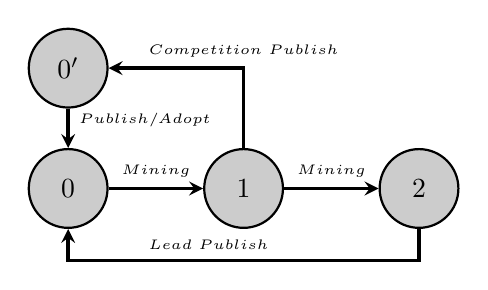
\begin{tikzpicture}
    \node[sm circ] (0) {$0$};
    \node[sm circ] (1)[right=1.2cm of 0] {$1$};
    \node[sm circ] (2)[right=1.2cm of 1] {$2$};
    \node[sm circ] (4)[above=0.5cm of 0] {$0^{\prime}$};

   	\draw [arrow] (0.east) -- node[pos= 0.5, anchor=south] {\tiny $Mining$}(1.west);
   	\draw [arrow] (1.north) |- node[pos=0.5, anchor=south] {\tiny $Competition$ $Publish$}(4.east);
   	\draw [arrow] (2.south) -- +(0,-0.4) -| node[pos=0.3, anchor=south] {\tiny $Lead$ $Publish$}(0);
   	\draw [arrow] (1.east) -- node[pos= 0.5, anchor=south] {\tiny $Mining$}(2.west);
   	\draw [arrow] (4) -- node[pos=0.3,anchor=west] {\tiny $Publish/Adopt$}(0);
   	
\end{tikzpicture}
}
\end{center}
   \caption{Abstract representation of state transtitions of eyal and sirer model for one selfish miner}
\label{fig:eyal_model}

\end{figure}
For clarification the state space and actions are modelled in \ref{fig:eyal_model}. The numbers in the states indicate the lead of the private to the public chain. $s$ denotes the lead of the private chain compared to the public chain. We can identify a total of four different actions.
\begin{itemize}
\item $Mining$: This action means that the peer has mined block. Mining adds the block to the private chain. It therefore causes $s$ to increase.
\item $Lead$ $Publish$: When $s$ increases to 2, the selfish miner will publish his private chain. It therefore causes $s$ to change from 2 to 0.
\item $Competition$ $Publish$: When $s$ is 1 and the selfish miner receives a block from another peer, he will publish his block of the same height from the private chain instead of the received one, to compete against the other miner. This causes a state transition to $0'$.
\item $Publish$: If the selfish miner is in state $0'$, he is in a competition situation.
The selfish miner will immediately publish his next mined block. This will cause the selfish miner to transition to state $0$.
\item $Adopt$: The selfish miner will adopt the main chain once he receives a new block in a competition situation.
\end{itemize}

\subsection{Gopalan Model}\label{gopalan}
The model of \citeauthor{gopalan} consists of a set of peers $P$ connected through a peer-to-peer network. Peers add blocks to the blockchain through a process called mining. 

The peer-to-peer network is modelled as an undirected Graph $H = (V,E)$.
An edge $(i,j) \in E$ represents communication possibilities between $v_i \in V$ and $v_j \in V$. 
The set of vertices is finite, such that $|V|=N \in \mathbb{N}$.
Vertices are associated with peers, such that $v_i$ represents peer $p_i \in P$.

Additionally, a directed acyclic graph $G_{p_i}(t) = (B_{G_{p_i}}(t),E_{G_{p_i}}(t))$ is associated with each peer $p_i$, at each point in time $t \in \mathbb{R+}$.
The vertex set $B_{G_{p_i}}(t) \subset \mathbb{N}$ represents the blocks known of peer $p_i$ at time $t$. The associated edge set of $E_{G_{p_i}}(t)$ represents references between blocks.
The following holds true for shorter notations:
\begin{equation}
B_G(t) = \cup_{i=1}^N B_{G_{p_i}}(t) \texttt{ and } E_G(t) = \cup_{i=1}^N E_{G_{p_i}}(t)
\end{equation}

Furthermore, the following equations hold for the principle of blockchains:
\begin{equation}
\forall p \in P: G_{p_i}(0) = (\{0\},\emptyset)
\label{genesis}
\end{equation}
\begin{equation}
t_1 < t_2 \rightarrow B_{G_{p_i}}(t_1) \subseteq B_{G_{p_i}}(t_2)
\label{nodegrow}
\end{equation}
\begin{equation}
t_1 < t_2 \rightarrow E_{G_{p_i}}(t_1) \subseteq E_{G_{p_i}}(t_2)
\label{edgegrow}
\end{equation}

Note that in this representation $0$ denotes the genesis block described in equation~\ref{genesis}.

$G_{p_i}(t)$ evolves over time. Blocks arrive over continuous time according to a stationary point process $A$ with intensity $\lambda$. Each block $b \in \mathbb{N}$ arrives at a random peer $p_i$.
This models peer $p_i$ mining block $b$ at time $t$ and that at this time the block is also added to $B_{G_{p_i}}(t)$.

References are added to $E_{G_{p_i}}(t)$ according to policy and depending on $G_{p_i}(t^-)$, where $t^-$ is a moment in time infinitesimally before $t$. $O_i$ denotes the set of outgoing neighbors of block $i$.

The communication is modelled as a marked point process $T_{p_i}$.
Each mark corresponds to another peer $p_j \in P\backslash \{p_i\}$.
In an epoch peer $p_i$ contacts $p_j$ and thus, adds the lowest numbered block of $B_{p_i}(t)\backslash B_{p_j}(t)$ to the set of Vertices $B_{p_j}$. If $B_{p_i}(t)\backslash B_{p_j}(t)$ is not empty, $E_{p_j}$ is also updated accordingly.

The peer-to-peer network dynamics are modelled as a continuous time rumor-spreading process with exogenous arrivals~\citep{gopalan}. Since communication is bound to the process $T_{p_i}$, the block dissemination is bandwidth limited.
Reference selection and thus $O_{p_i}$ is chosen accordant to longest chain policies~\citep{gopalan}.

Let $L_{p_i}(t)$ denote the set of nodes farthest away from the genesis block $0$, known to peer $p_i$ at time $t$.
\begin{equation}
L_{p_i}(t) := \{j \in B_{p_i}(t): d(j,0)\geq d(j',0), \forall j' \in B_{p_i}(t) \}
\label{policy}
\end{equation}

Note that the set $O_{p_i} \cap L_{p_i}(t)$ is non empty. This constructs a simple directed acyclic graph. The Tree Policy~\citep{gopalan} can then be determined as $|O_{p_i}|=1$ and establishes the following relationship:
\begin{equation}
|E_{G_{p_i}}(t)| = |B_{G_{p_i}}(t)| -1
\end{equation}
Every block will have exactly one outgoing reference, according to some deterministic rule~\citep{gopalan}. \citeauthor{gopalan} assume that the block with the lower index number will be chosen.


\subsection{ extension -- selfish mining inclusion}\label{selfishmodel}
The selfish mining attack is described as a peer executing a protocol deviant from honest mining~\citep{eyal}. Therefore a selfish miner can be modelled according to the model described in \ref{gopalan} through altering the reference selection and communication process. The reference selection process is policy driven, and can thus be modified by providing a new selfish policy. 

Peer $SM \in P$ has an associated policy slightly different to \ref{policy}. Note that to follow the Tree Policy~\citep{gopalan}, a deterministic rule has to be established for the case that $|O_{SM} \cap L_{SM}(t)| > 1$.

Assume that $SM$ has the knowledge of the set of blocks mined through him, $M_{SM}(t) \subset B_{G_{SM}}(t)$. $SM$ will set 
\begin{equation}
(L_{SM}(t) \cap M_{SM}(t)) \neq \emptyset \rightarrow L'_{SM}(t) \subset ( L_{SM}(t) \cap M_{SM}(t)) 
\label{smpolicy}
\end{equation}
It then follows that $|L'_{SM}(t)|=1$.
This modified tree policy sets references according to the original selfish mining protocol described by \citeauthor{eyal}.

The second aspect to be modified is the communication process. 
Key idea of selfish mining is block withholding. The selfish miner possesses three blockchain representations. 
\begin{itemize}
\item $G_{SM_{public}}(t)$: which is updated by other peers.
\item $G_{SM_{comm}}(t)$: which is used to update other peers.
\item $G_{SM_{private}}(t)$: with the following relations:
		\begin{itemize}
		\item $G_{SM_{public}}(t)\subseteq G_{SM_{private}}(t)$.
		\item $G_{SM_{private}}(t)\backslash G_{SM_{public}}(t)$ represents blocks mined but unpublished by the selfish miner.
\end{itemize}		
\end{itemize}


\begin{figure}
\begin{center}
\resizebox{\columnwidth}{!}{%
  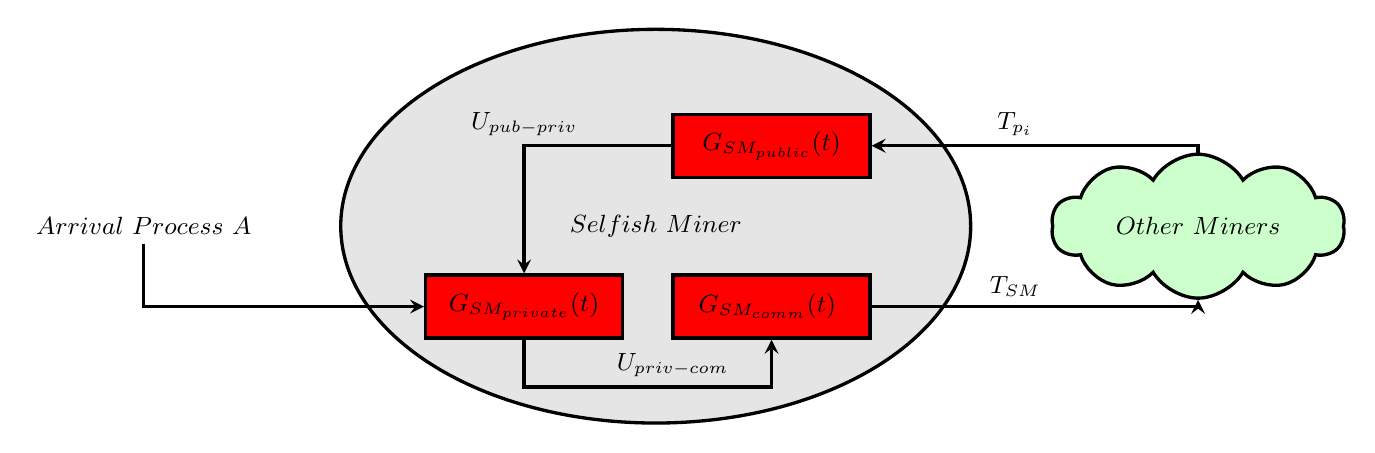
\begin{tikzpicture}
  \small
    \node[sm node] (1) {$Selfish~Miner$};
    \node(2) [left = 1cm of 1] {$Arrival~Process~A$};
    
    \node[block] (3) [above right = 0.6cm and 0.2cm]{$G_{SM_{public}}(t)$};
    \node[block] (5) [ below =1.2cm of 3 ]{ $G_{SM_{comm}}(t)$ };
	\node[block] (4) [left=0.6cm of 5]{$G_{SM_{private}}(t)$};    
    
    \node [cloud,fill=green!20, draw,very thick,cloud puffs=10,cloud puff arc=120, aspect=3, inner ysep=1em, right=1cm of 1](6) {$Other~Miners$};
    
   	
   	\draw [arrow] (2) |- (4);
   	\draw [arrow] (3) -| node[anchor=south] {$U_{pub-priv}$}(4);
   	\draw [arrow] (4.south) -- +(0,-0.6) -| node[pos=0.3, anchor=south] {$U_{priv-com}$}(5);
   	\draw [arrow] (6) |- node[pos=0.78,anchor=south] {$T_{p_i}$}(3);
	\draw [arrow] (5) -| node[pos=0.22,anchor=south] {$T_{SM}$}(6);    
\end{tikzpicture}
}
\end{center}
   \caption{Abstract representation of model entities and communication processes}
\label{fig:model_vis}

\end{figure}
The concept has been visualized in \ref{fig:model_vis}.
A total number of five processes is used to let all entities interact with each other.
\begin{itemize}
\item $Arrival~Process~A$: Blocks arrive to the selfish miner over the external arrival process $A$.

\item $T_{p_i}$: Ensures blocks from other peers are communicated to $G_{SM_{public}}(t)$.
\item $U_{pub-priv}$: Ensures that $G_{SM_{public}}(t)\subseteq G_{SM_{private}}(t)$ holds true, meaning $U_{pub-priv}$ updates $G_{SM_{private}}(t)$, when new blocks arrive to $G_{SM_{public}}(t)$ from other peers.
\item $U_{priv-com}$: Updates $G_{SM_{comm}}(t)$ according to $G_{SM_{private}}(t)$ and the selfish mining rules $S$.

\item $T_{SM}$: Ensures other peers are updated with blocks from $G_{SM_{comm}}(t)$.

\end{itemize}

$S$ is a set of rules which describes how $G_{SM_{private}}(t)$ updates $G_{SM_{comm}}(t)$. The rules have to follow the state description of \citeauthor{eyal}\ref{eyalmodel}. Therefore we need a state variable describing the difference between private and public chain.
Let $s$ be the state variable determining selfish mining actions~\citep{eyal}.
Then $s$ can be described as a difference between $G_{SM_{private}}(t)$ and $G_{SM_{public}}(t)$.
\begin{equation}
max\_ dist(G_{p_i}(t)) := d(j,0), j \in L_{p_i}(t)
\end{equation}
\begin{equation}
max\_ dist\_mined(G_{p_i}(t)) := d(j,0), j \in M_{p_i}(t)
\end{equation}
\begin{equation}
s(t) := max\_ dist(G_{SM_{private}}(t)) - max\_ dist(G_{SM_{public}}(t))
\end{equation}
\begin{equation}
s_{mined}(t) := max\_ dist\_mined(G_{SM_{private}}(t)) - max\_ dist(G_{SM_{public}}(t))
\end{equation}
Let $t_{inc}$ refer to the set of times, where $s$ increased and analogous $t_{dec}$ refer to the set of times, where $s$ decreased.
Additionally, let $t'_{inc}$ refer to the set of times, where $s_{mined}$ increased and analogous $t'_{dec}$ refer to the set of times, where $s_{mined}$ decreased.
Note that $s>0$, because $G_{SM_{public}}(t) \subseteq G_{SM_{private}}(t)$.
Let $f_{-1}(t)$ be a function that outputs the point in time, where s changed the latest before $t$.
$U_{priv-com}$ can then be characterized through four kind of update actions. Analogous to Subsection\ref{eyalmodel}, those actions are $Lead~Publish$, $Competition~Publish$, $Publish$ and $Adopt$. $Mining$, the fifth action described in Subsection\ref{eyalmodel}, is modelled through the arrival process.
This can be used to model the selfish mining protocol desribed by \citeauthor{eyal}.
\begin{enumerate}
\item $Lead~Publish$: Assume $t \in t_{inc}$ and $s(t) \geq 2$, then $U_{priv-com}$ updates $G_{SM_{comm}}(t)$, such that $G_{SM_{comm}}(t) = G_{SM_{private}}(t)$. 
\item $Competition~Publish$: Assume $t \in t_{dec}$, $s(t) = 0$, $s(f_{-1}(t)) = 1$, $s(f_{-1}(t)^-) = 0$. This means that the selfish miner mined a block, did not publish it and now received a block from another of the same height. This leads to the competition scenario. Accordingly, $U_{priv-com}$ updates $G_{SM_{comm}}(t)$, such that it includes the subgraph induced by the nodes on the paths between $L'_{SM}(t)$ and ${0}$. This transitions to 
\begin{equation}
0'(t) \rightarrow \left( t \in t_{dec} \wedge s(t) = 0 \wedge s(f_{-1}(t)) = 1 \wedge s(f_{-1}(t)^-) = 0\right)
\end{equation}
\item $Publish$: Assume $0'(t^-)=\top$ and $t \in t_{inc}$, $U_{priv-com}$ updates $G_{SM_{comm}}(t)$, such that it includes the subgraph induced by the nodes on the paths between $L'_{SM}(t)$ and ${0}$.
\item $Adopt$: Assume $0'(t^-)=\top$ and $s'(t)=-1$, then $U_{priv-com}$ updates $G_{SM_{comm}}(t)$, such that $G_{SM_{comm}}(t) = G_{SM_{private}}(t)$. 

\end{enumerate}










\chapter{Contribution}\label{chap:contribution}
T
Therefore, the model proposed by \citeauthor{gopalan} has been enhanced to model selfish mining behaviour in \ref{selfishmodel}.
The relationship between selfish mining and networking effects can be charactized by a number of key questions.
Those questions can be split up in two groups.
The first group considers how the network influences selfish mining.
Key aspects include:
\begin{enumerate}
\item \citet{xiao_modeling} show in their model that revenue gain and profitability threshhold correlates to betweenness centrality. Does this correlation also show \ref{selfishmodel}?
\item Does a networking advantage increase revenue gain and profitability threshhold?
\item Does a certain network topology influence selfish mining effectiveness?
\end{enumerate}
The second group considers how selfish mining influences the network.
Key aspects include:
\begin{enumerate}
\item Does the network have a different throughput, if one peer is executing the selfish mining protocol?
\item Does the network have a different block propagation time, if one peer is executing the selfish mining protocol?
\item Does the network show different congestion peeks, if one peer is executing the selfish mining protocol?
\item If the network shows congestion peeks, does it correlate to certain actions the selfish miner is performing?
\end{enumerate}
´







\chapter{Evaluation}\label{chap:evaluation}
The following section utilizes the simulative implementation of the Blockchain Gossip Model to evaluate the relationship between selfish mining and networking effects. Additionally, the model will be validated against data provided by \gopalan and real world data of the Bitcoin system.
\section{Simpy Blockchain Simulator}
The core implementation is based on simpy~\cite{simpy}. Simpy is a discrete event simulator written in python. As a result the Simpy Blockchain Simulator is also written in python. 
The Selfish Rumor Model consists mainly of four parts. 
\begin{itemize}
\item Networkgraph representation
\item Blockchain representation
\item Block Arrival Process representation
\item Communication Process representation
\end{itemize}
The network graph is represented by an adjacency matrix. The blockchain representation is a set of blocks and a set of edges for each peer, which are developing over time. The block arrival process and the communication process are modelled as a Poisson process~\cite{poisson}. This is mirrored in a Simpy process with an exponentially distributed interarrival time between scheduled events.
On each event of the block arrival process a block arrives at a random peer. This means that the event triggered by the block arrival process updates the blockchain datastructure accordingly.
At each event of the communication process $T_i$ a peer $p_i$ tries to update a certain peer $p_j$ according to the epoch associated with the event. This results in a comparison between the datastructures associated with $p_i$ and $p_j$ and an update of $p_j$, if it is possible.

Even though the basic implementation is simple, there are various parameters which influence the system behaviour greatly. The following list shall give an overview:
\begin{itemize}
\item Average of interarrival times - This is the rate of block arrival process and communication process trigger events. 
\item Topology of the network graph - The network resulting from the adjacency matrix has a great influence on the bahviour of the system.
\item Block selection - In a scenario, where multiple blocks could be transferred from one peer to another, one block has to be selected. How this block is selected influences system baviour.
\item Network size - This is the number of peers.
\item Mining power distribution - The mining power distribution influences the peer selection. Peer selection is the process of deciding which peer gets the new block once the block arrival process triggers an event.
\end{itemize}
The above discussed parameters can be modified in order to capture different systems.

\section{Validation of the Simpy Blockchain Simulator}
In the following section the Simpy Blockchain Simulator is validated against synthetic experiments published by the original authors of the blockchain gossip model. Additionally real world data from Bitcoin will be additionally used to validate the legitimacy of the Simpy Blockchain Simulator. This will lay the fundamant for further analysis concerning the network and selfish mining. 
\subsection{Validation of Simulator against \gopalan}\label{gopalananalysis}
In the synthetic data experiments of \gopalan~  they analyze the the network for 10, 20 and 30 peers. The network topology is a complete graph. Thus, the adjacency matrix is the unit matrix. 
The authors introduce four key metrics to analyze the system. Those are 
\begin{itemize}
\item Time to Consistency --- The average time an inconsistent system needs to reach a state of consistency
\item Cycle Length --- The sum of the average time to consistency and the average of the time the system stays consistent
\item Consistency Fraction --- The average fraction of peers that are consistent at each point in time
\item Age of Information --- The average number of blocks an average peer is away from the consistency state
\end{itemize}
All metrics mentioned above refer to the term consistency. The Consistency is defined as $B_G(t)$~\ref{unisondef}, the unison of all blocks produced by the block arrival process $A$.
In order to evaluate to capture the same system, that was analyzed by the authors, the parameters are setup similar.
These metrics can be used to verify whether the Simpy Blockchain Simulator is achieving similar numbers to the implementation of \gopalan . 
\begin{itemize}
\item Average of interarrival times - The interarrival time of the communication process is set to 1s. The interarrival time of the block arrival process is a variable.
\item Topology of the network graph - The network topology is a complete graph.
\item Block selection - In a scenario, where multiple blocks could be transferred from one peer to another the block with the lowest index number is chosen.
\item Network size - The number of peers is set to 10, 20 and 30 accordingly.
\item Mining power distribution - The mining power distribution is uniform.
\end{itemize}

\begin{figure}[h]
	\begin{subfigure}[b]{0.48\textwidth}
		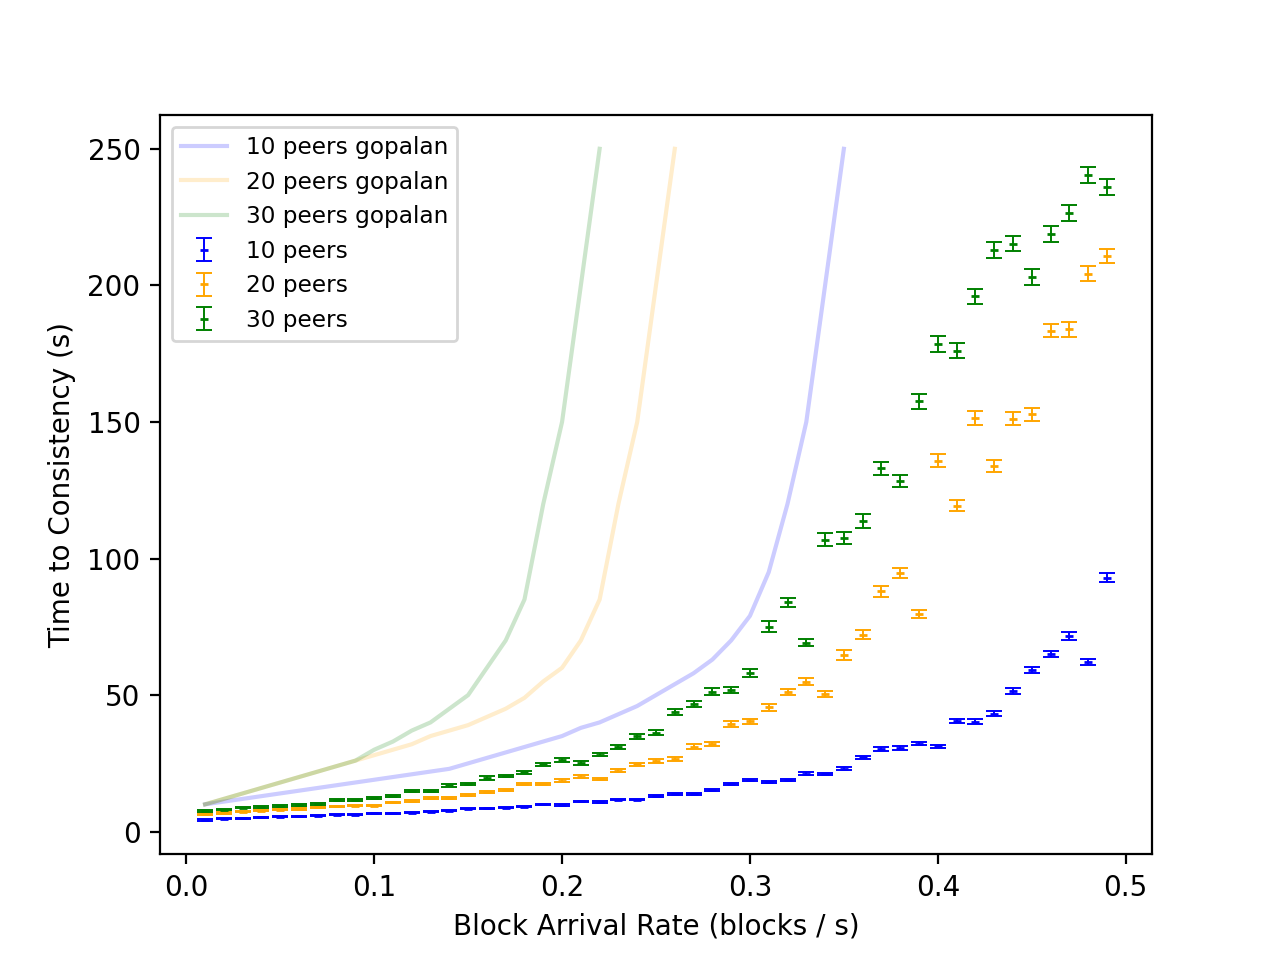
\includegraphics[width=\textwidth]{figures/gopalan_figures/time_to_consistency.png}
		\caption{ Time to Consistency}
		\label{fig:gopalan_ttc}
	\end{subfigure}
	\hfill
	\begin{subfigure}[b]{0.48\textwidth}
		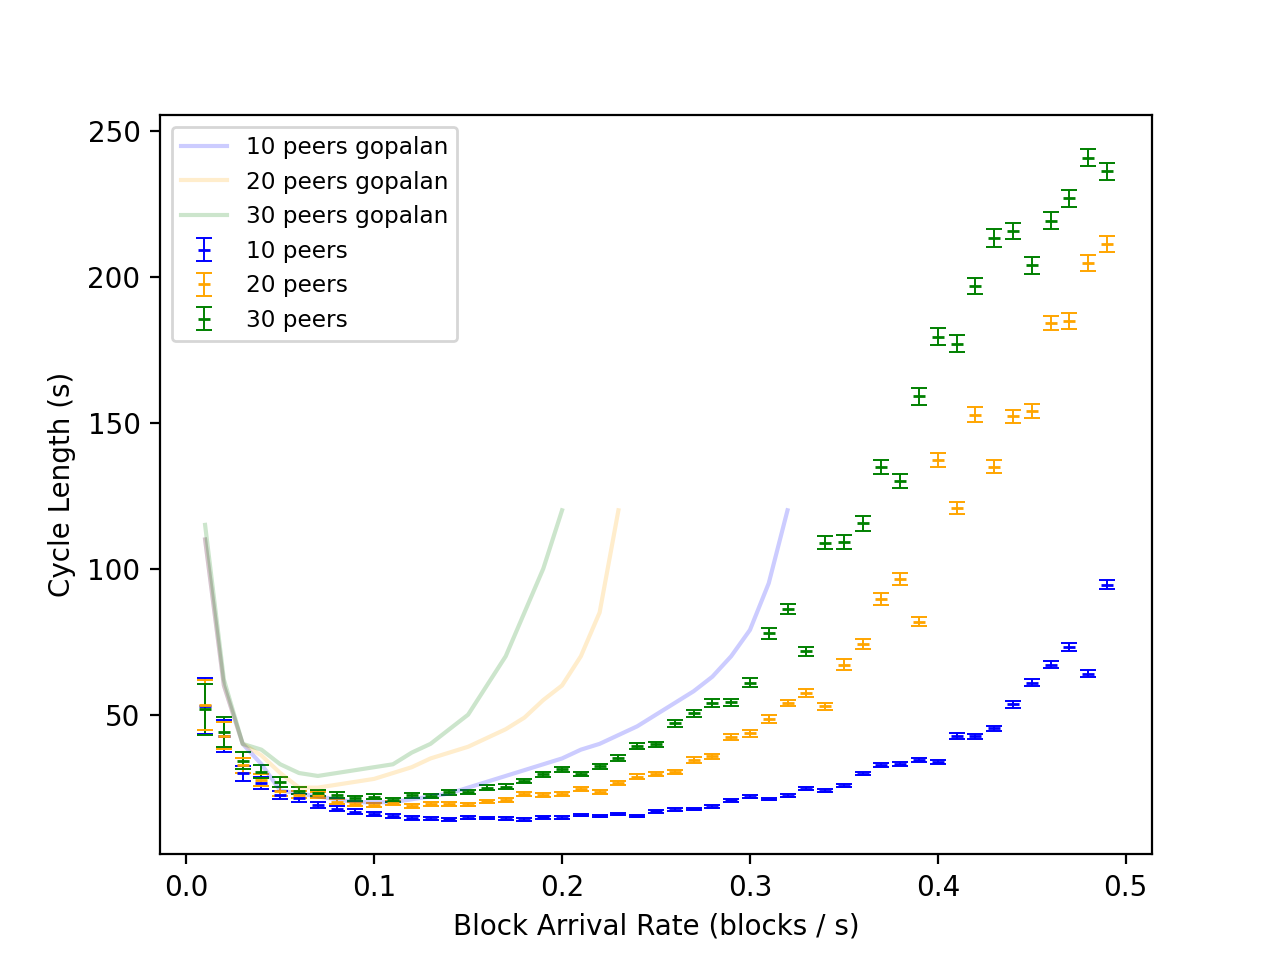
\includegraphics[width=\textwidth]{figures/gopalan_figures/cycle_length_avg.png}
		\caption{ Cycle Length}
		\label{fig:gopalan_cl}
	\end{subfigure}
	\hfill
	\begin{subfigure}[b]{0.48\textwidth}
		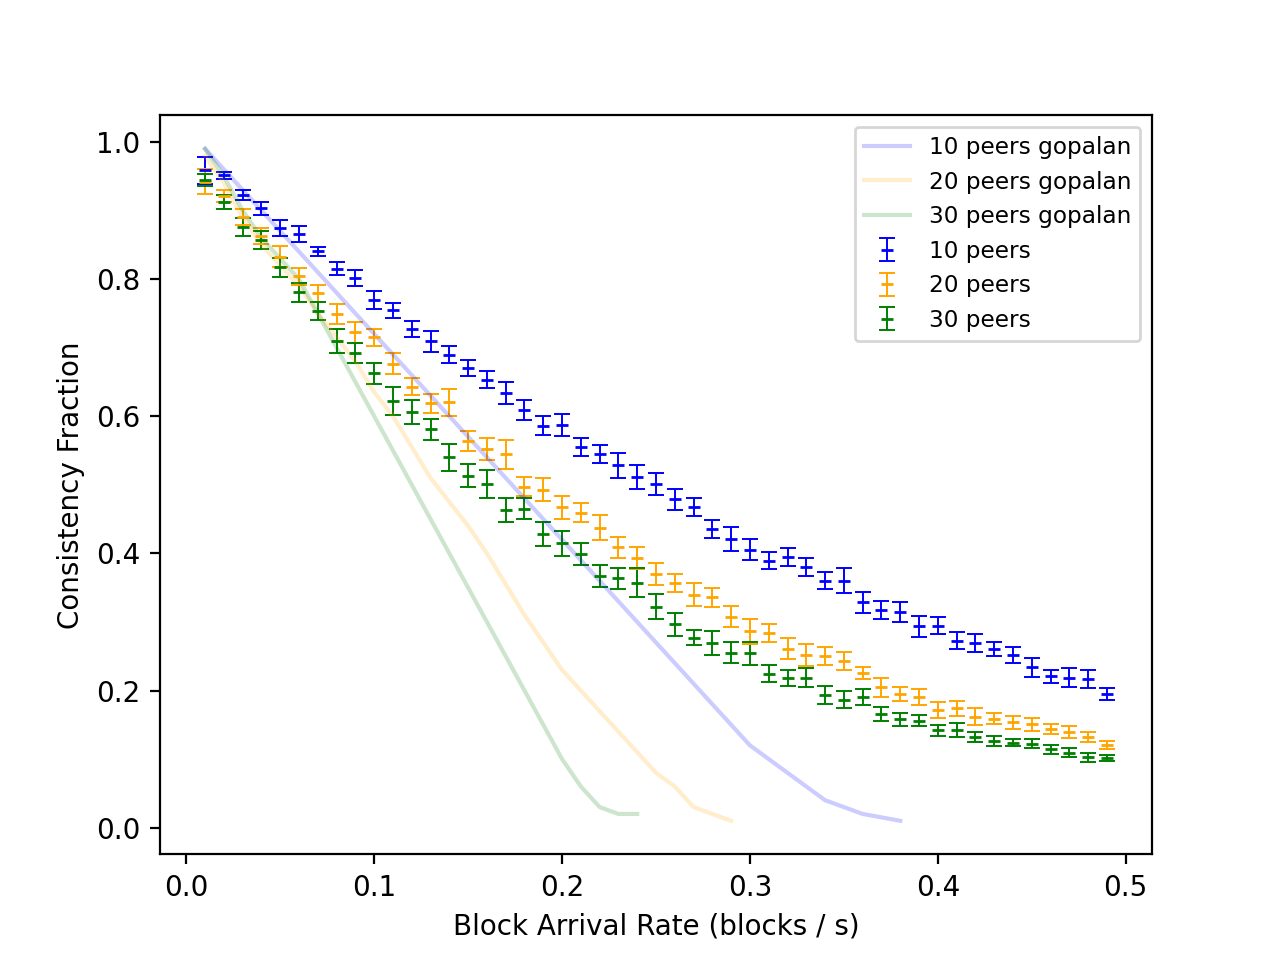
\includegraphics[width=\textwidth]{figures/gopalan_figures/consistency_fraction.png}
		\caption{ Consistency Fraction}
		\label{fig:gopalan_cf}
	\end{subfigure}
	\hfill
	\begin{subfigure}[b]{0.48\textwidth}
		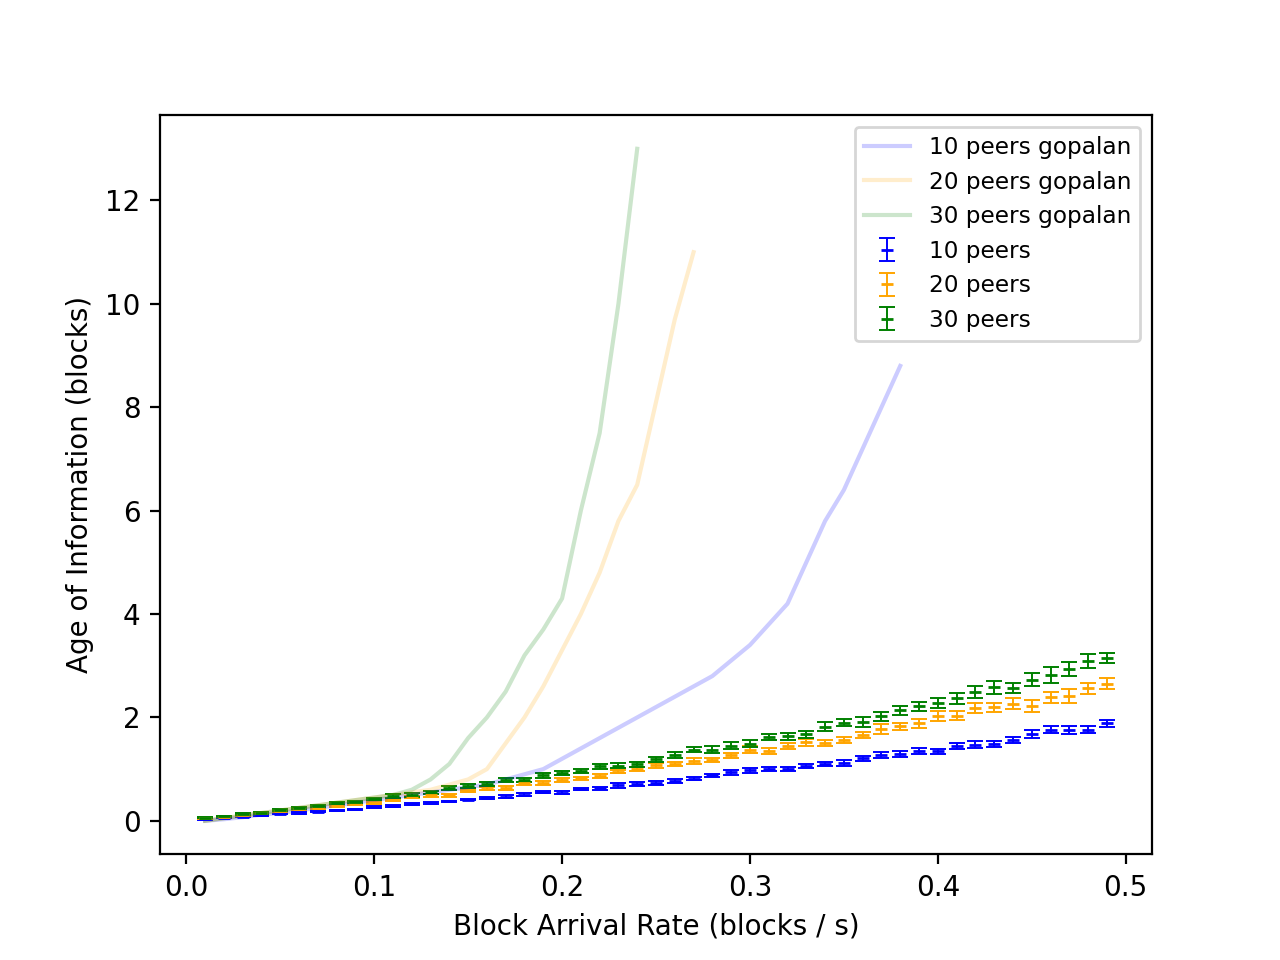
\includegraphics[width=\textwidth]{figures/gopalan_figures/age_of_information.png}
		\caption{ Age of Information}
		\label{fig:gopalan_aof}
	\end{subfigure}
	\caption{Comparison between Simpy Blockchain Simulator and values produced by \gopalan}
\end{figure} 

The metrics of time to consistency and cycle length are very closely related, because both rely on the time the system needs to reach consistency.
Figure~\ref{fig:gopalan_ttc} and Figure~\ref{fig:gopalan_cl} show this close relationship. Additionally the comparison between the Simpy BLockchain Simulator shows a very similar tendency in both metrics. Especially in Figure~\ref{fig:gopalan_ttc} it is observable that the curve has the same shape, only flatter. Figure~\ref{fig:gopalan_ttc} shows that peernumber and block arrival rate are proportional to the average time to consistency. Since cycle c´ength is the sum of the average time to consistency and the average of the time the system stays consistent the same behavior can be observed in Figure~\ref{fig:gopalan_cl}. Additionally Figure~\ref{fig:gopalan_cl} shows that for very small numbers for the block arrival rate the cycle length increases again. When the system has a low block arrival rate the system tends to stay longer in a state of consistency, which is due to the fact that the idle time increases.

Consistency fraction and age of information are both metrics measuring the consistency of an average peer. The consistency fraction is the fraction of peers, which have a blockset equal to $B_G(t)$~\ref{unisondef}. For both the simulation results by \gopalan~ and the Simpy Blockchain Simulator we can observe, that the consistency fraction decreases with an increasing blockrate and peer number. While the exact numbers do differ, similar shapes can again be observed.
The age of information metric analyzes how much an average peer differs from $B_G(t)$~\ref{unisondef}. It showcases an increase for an increasing blockrate and peer number.

The differences indicate that information spreads faster in the Simpy Blockchain Simulator. After a brief discussion with \gopalan~, they confirmed that this might be due to the fact, that in the simpy version communication processes are handled truly concurrently.	

\subsection{Validation of Simulator against Bitcoin data}
This section validates the model against a real world blockchain system, the Bitcoin network. The Selfish Rumor Model implements an abstract network model of blockchain systems, simulating block creation and block propagation.
Researchers of the Karlsruher Institut für Technologie \cite{BitcoinNetworkMonitor} monitor the Bitcoin network and obtain data of, for example, the current block propagation delay distribution. Since the Model can be used to analyze blocks and their propagation, the current block propagation delay distribution is a suitable metric to compare the Selfish Rumor Model against the real world system.

\begin{figure}[ht]
	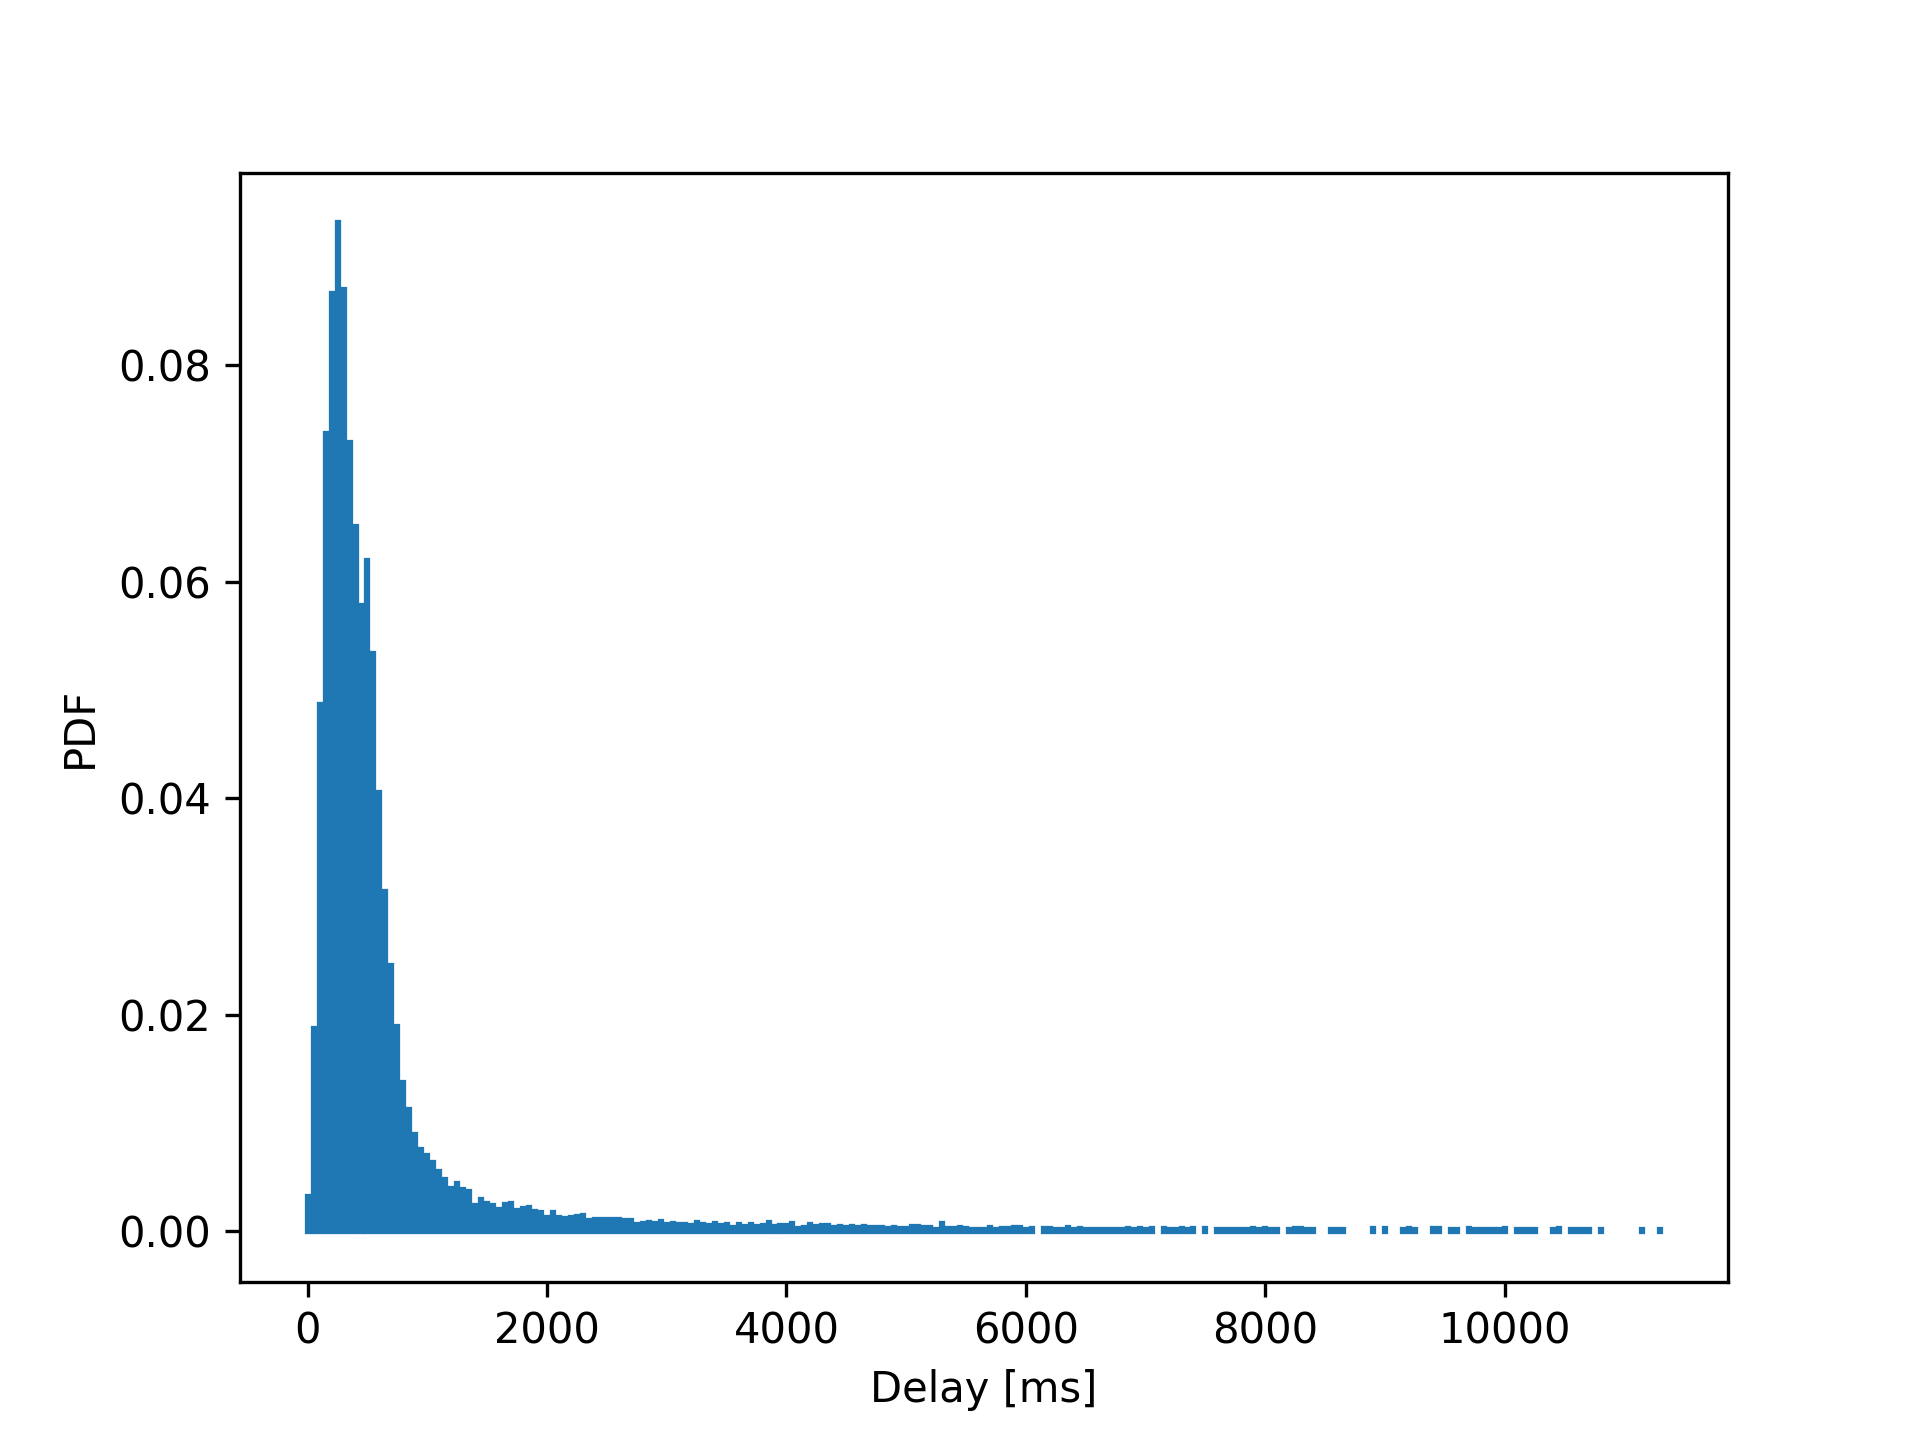
\includegraphics[width=\textwidth]{figures/bitcoin_current_block_propagation_delay_distribution.png}
	\caption{Bitcoin Current Block Propagation Delay Distribution \cite{BitcoinNetworkMonitor}}
	\label{fig:blockdelaydis}
\end{figure}
Figure~\ref{fig:blockdelaydis} visualizes the current block propagation delay distribution of Bitcoin. The $1\% $ of the largest delays have been filtered out and the data points have been grouped in $150ms$ steps. A significant characteristic seen in the plot is the high peek at $~400ms$ and the long tail going up to about $10000ms$ delay. Around $72\% $ of peers have a block propagation delay below $500ms$. Especially the long tail distribution is a very important characteristic for the current block propagation delay distribution.

With the characteristics obtained through the Bitcoin Network Monitor it is possible to search for a parameter setup for the Selfish Rumor Model, which mimics the block propagation characteristics of Bitcoin.
To achieve a similar block propagation one can analyze mainly the topology of the network graph and the communication process rate.

\begin{figure}[ht]
	\begin{subfigure}[b]{0.48\textwidth}
		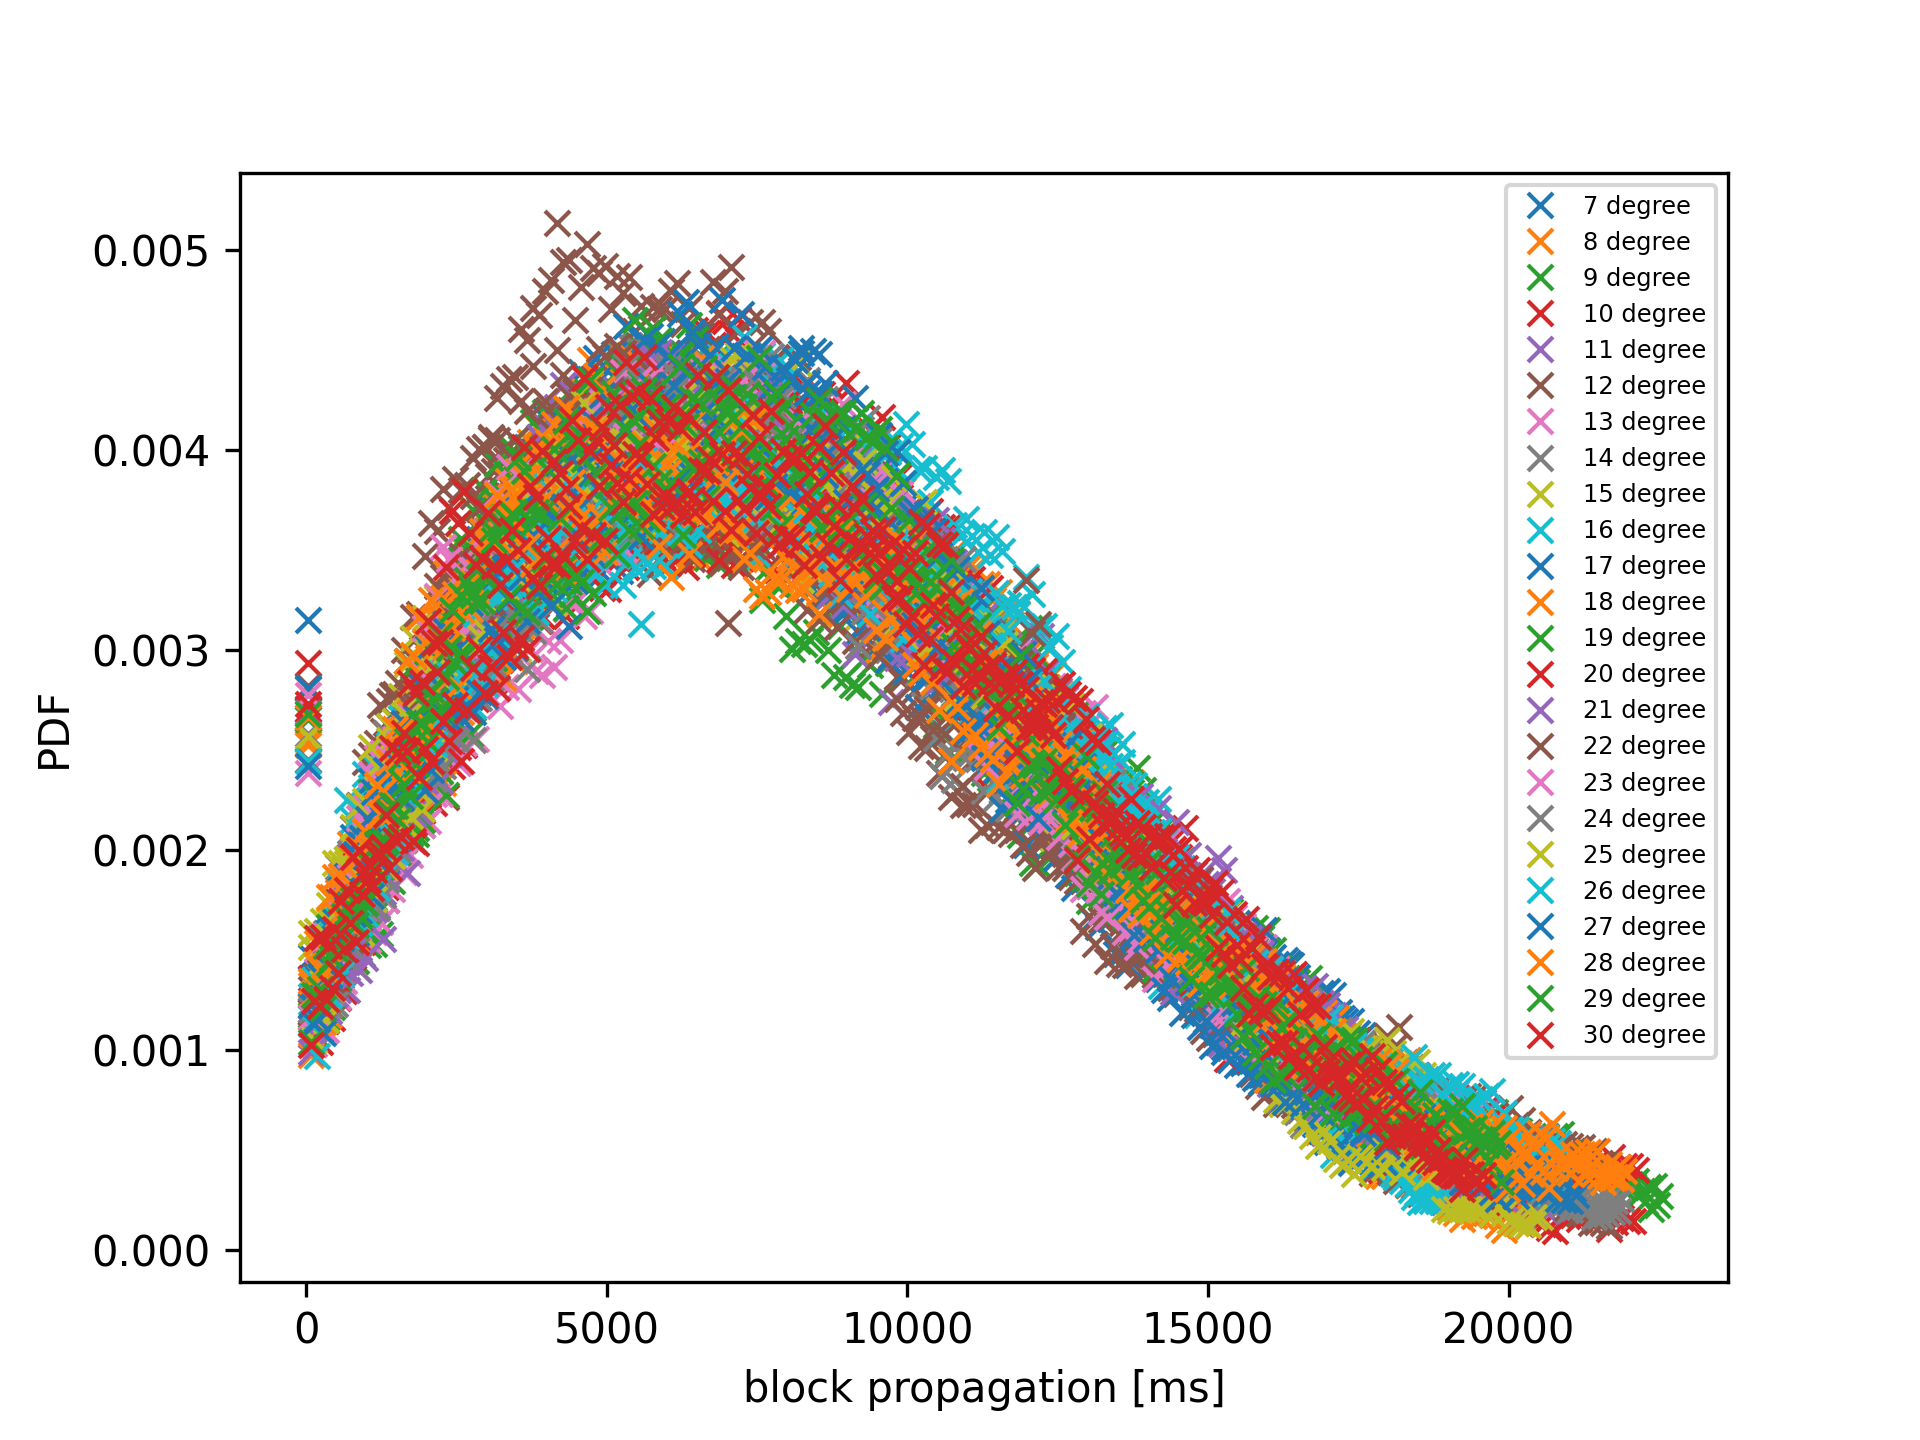
\includegraphics[width=\textwidth]{figures/propagation_histogram_degree_search_smaller.png}
		\caption{Block Propagation Delay Distribution }
		\label{fig:SRMblockprop}
	\end{subfigure}
	\hfill
	\begin{subfigure}[b]{0.48\textwidth}
		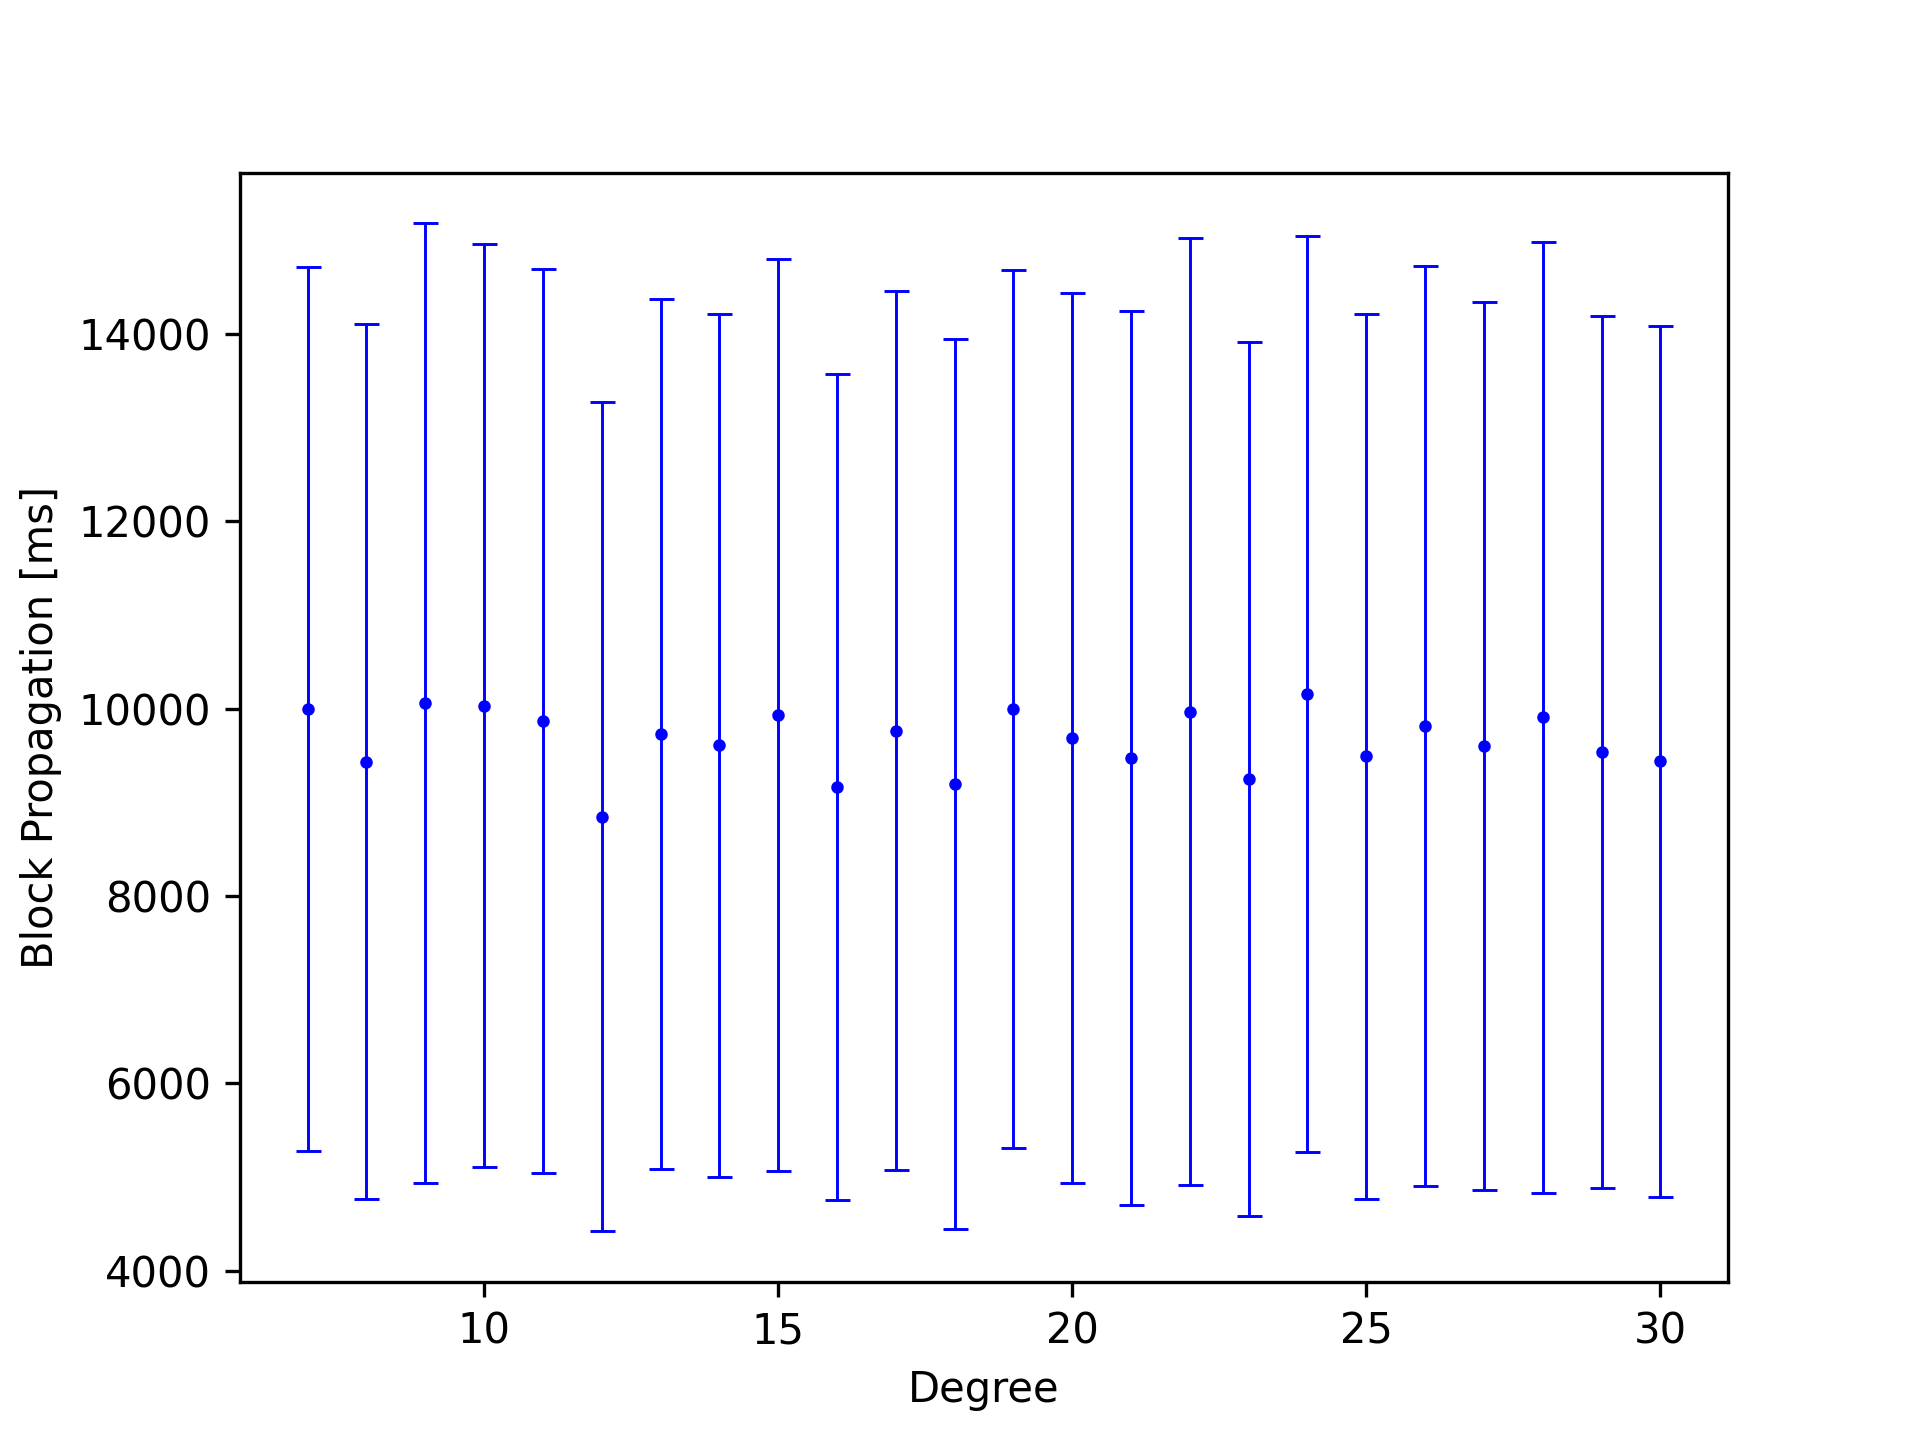
\includegraphics[width=\textwidth]{figures/avg_propagation_degree_search.png}
		\caption{Average Block Propagation Delay with standard deviation }
		\label{fig:SRMblockpropavg}
	\end{subfigure}
\caption{Selfish Rumor Model Experiments for various degrees in a regular-random graph, 500 peers, Communication process rate 1ms, Block Arrival Process rate 600s}
\end{figure}
Figure~\ref{fig:SRMblockprop} shows the block delay distribution for the selfish rumor model. The $1\% $ of the largest delays have been filtered out and the data points have been grouped in $50ms$ steps. Each parameter setup was simulated for 500 blocks and repeated fifty times with different seed values.
The shape of the distribution curve differs in shape and magnitude. The curve of the Selfish Rumor Model is wider and has a peak at around 6000ms.
Figure~\ref{fig:SRMblockpropavg} shows, that the average block propagation is around $10000ms$ independent of the selected degree. It also shows a high standard deviation and therefore a high variance.

The second modifiable parameter is the communication process rate.
\begin{figure}[ht]
	\begin{subfigure}[b]{0.48\textwidth}
		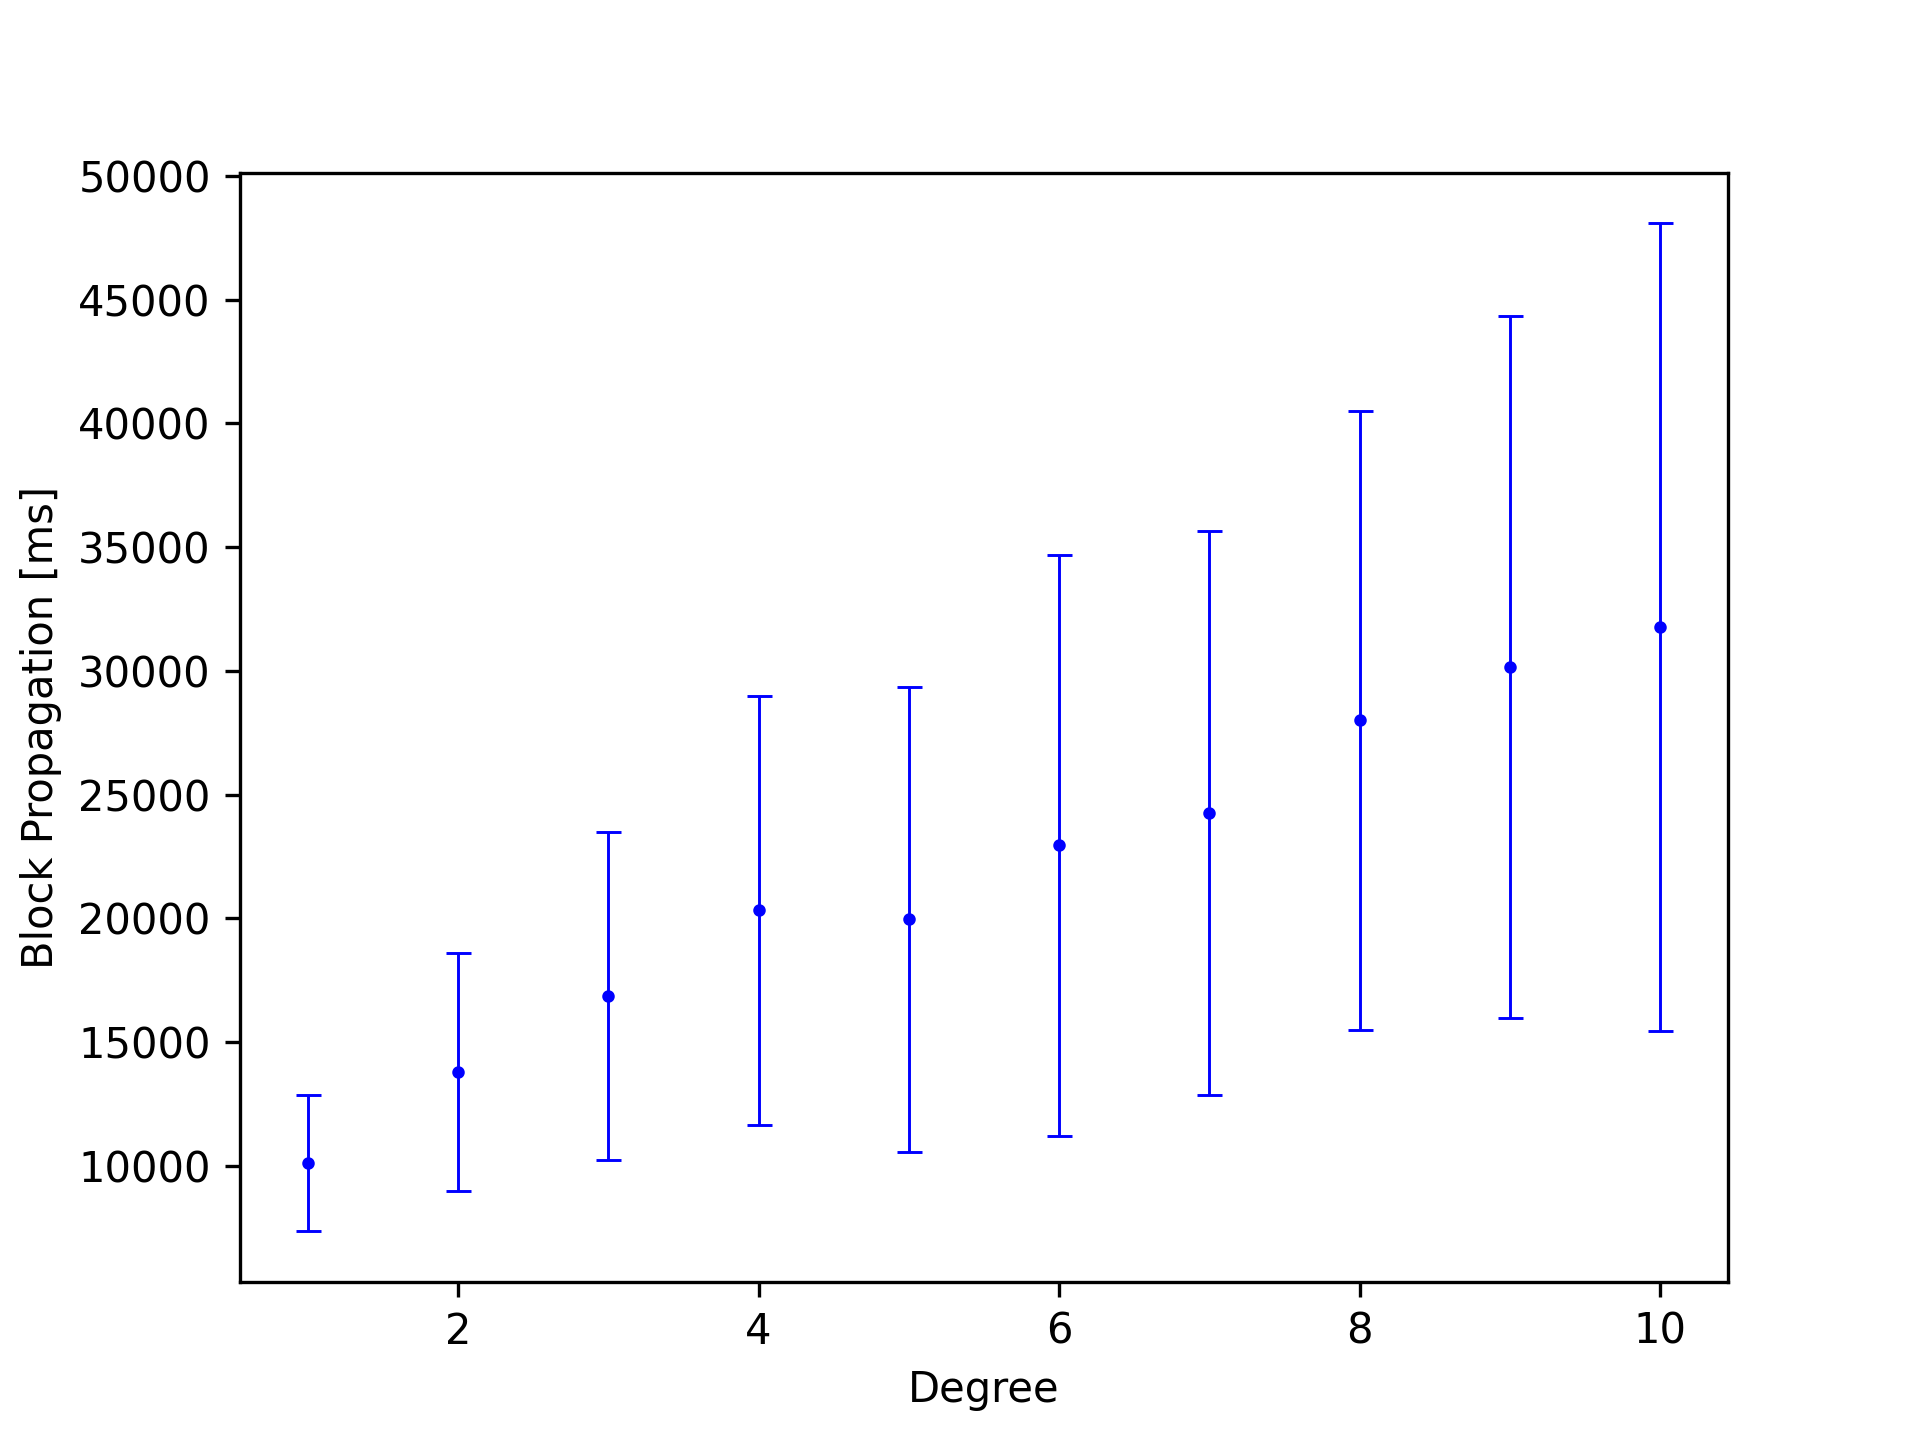
\includegraphics[width=\textwidth]{figures/avg_propagation_comm_rate_search.png}
		\caption{Regular Random Graph Degree 8}
		\label{fig:CommSearch8}
	\end{subfigure}
	\hfill
	\begin{subfigure}[b]{0.48\textwidth}
		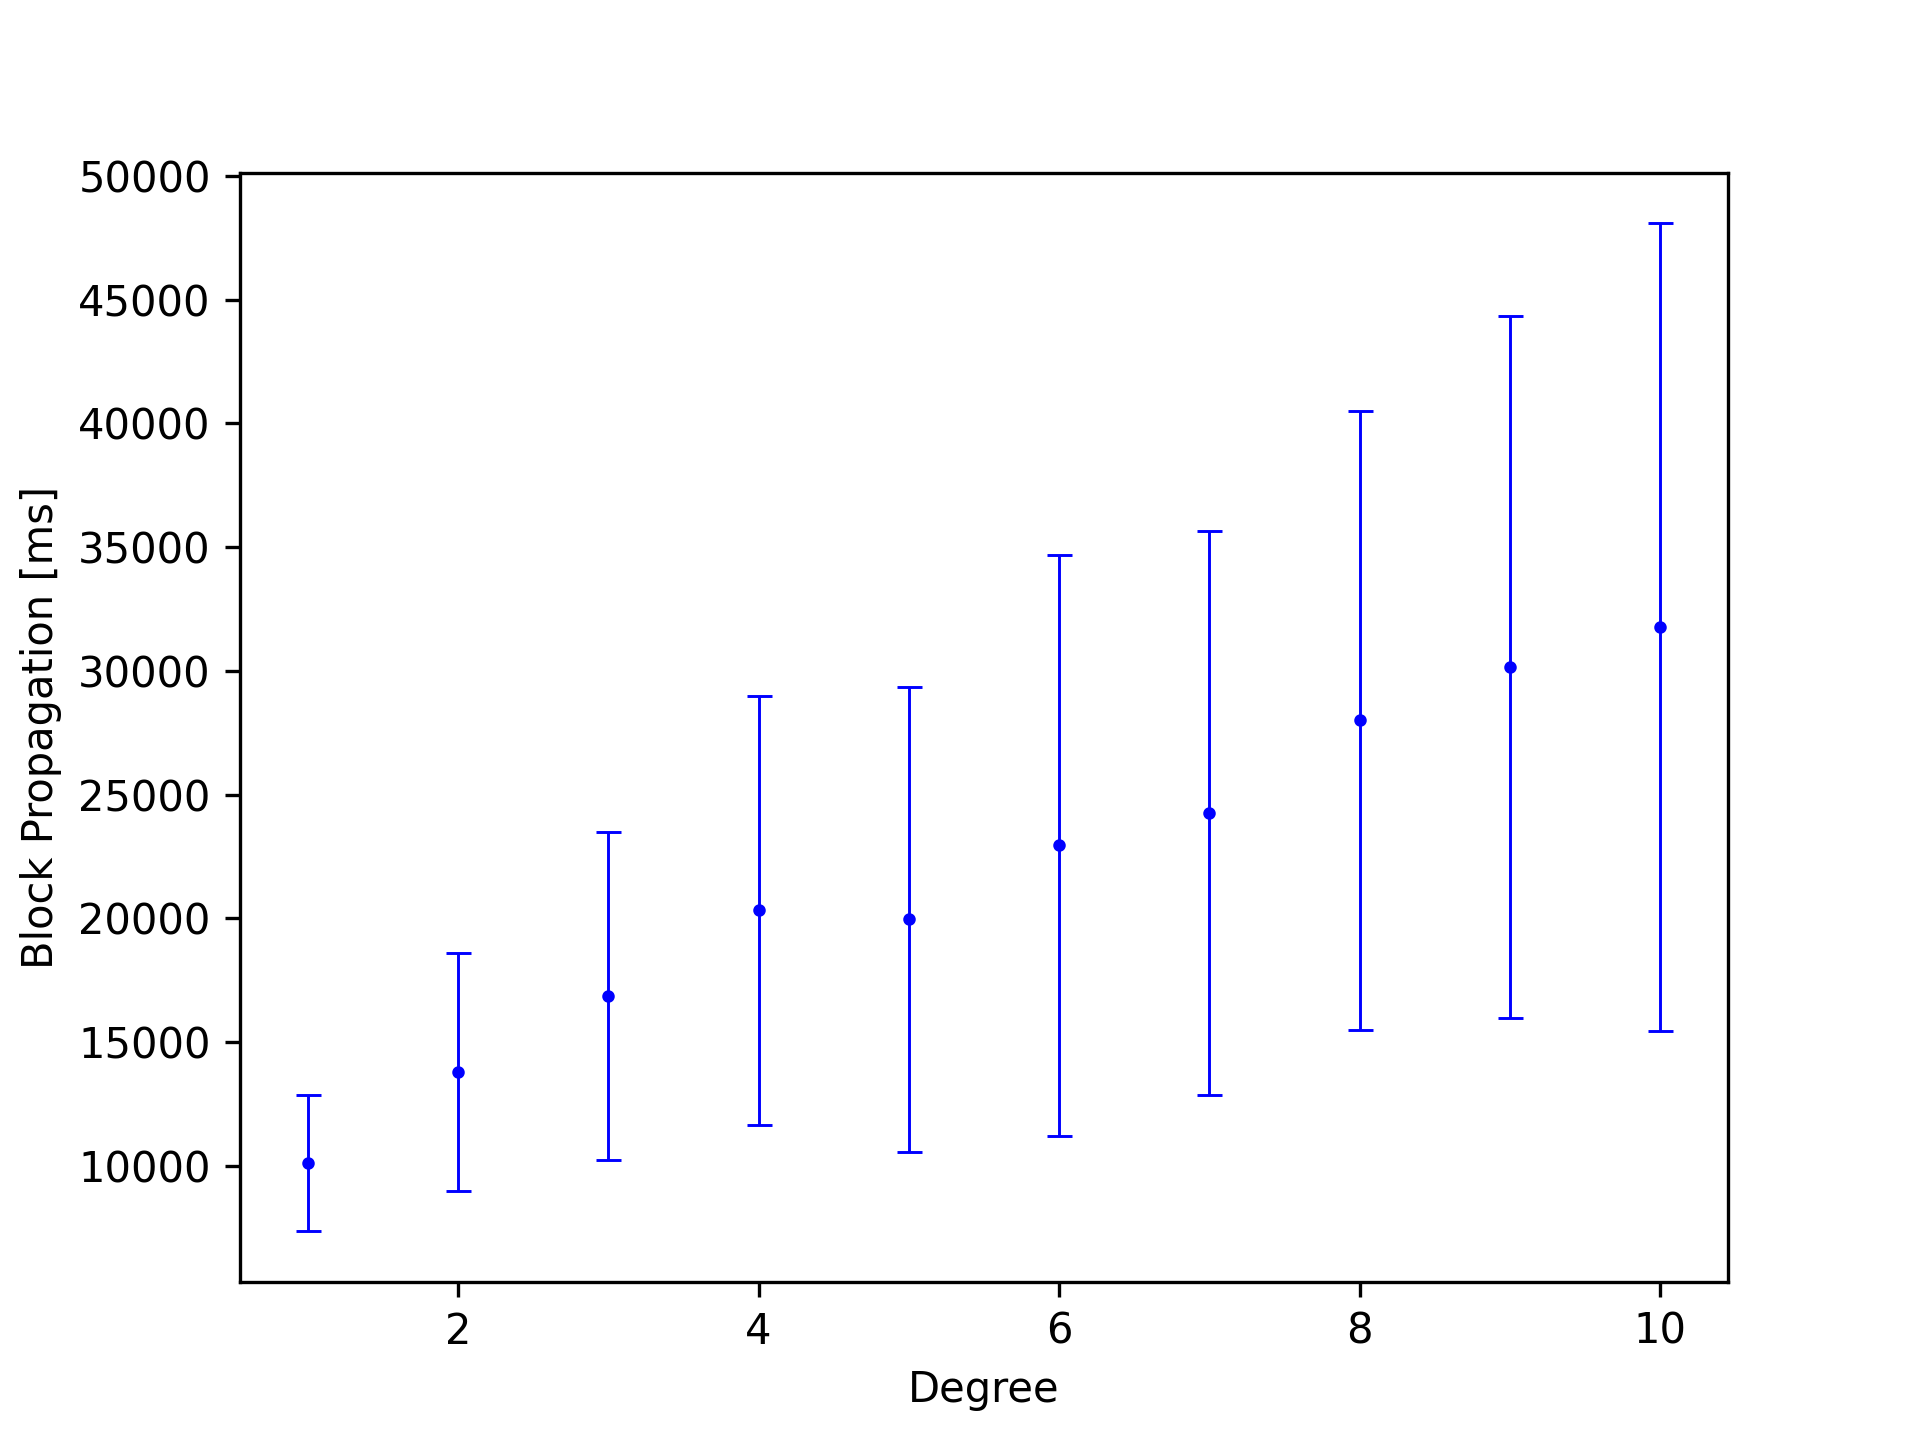
\includegraphics[width=\textwidth]{figures/avg_propagation_comm_rate_search.png}
		\caption{Regular Random Graph Degree 8 TODO 16}
		\label{fig:CommSearch16}
	\end{subfigure}
\caption{Selfish Rumor Model Experiments for various communication process rates in a regular-random graph, 500 peers, Block Arrival Process rate 600s}
\end{figure}
Figure~\ref{fig:CommSearch16} as well as Figure~\ref{fig:CommSearch8} both show a proportional relationship between the rate of the communication processes and block propagation time. 
TODO: Simulationen noch nicht durch 1-2 sätze zur genauen auswertung

The above simulations do not indicate a parameter setup to achieve a similar block propagation in the Selfish Rumor Model as in Bitcoin. This can be due to that fact that over the last years Bitcoin has seen numerous improvements towards achieving a faster block propagation time. Two of these improvements are Compact Blocks and the FIBRE Network respectively. However, it is not only the lower average block propagation time, but also the different shape of the curve. This indicates that an even more similar block propagation is not possible.
Additionally, reviewing older Bitcoin statistics \cauth{BlockPropOld} found an average block propagation of $12.6s$.

We conclude this section by establishing a parameter setup, denoted as Bitcoin Parameter setup. This parameter setup will be used to mimic a blockchain system as close as possible to Bitcoin.
\begin{itemize}
\item Average of interarrival times - The interarrival time of the communication process is set to 1ms. The interarrival time of the block arrival process is set to 600s.
\item Topology of the network graph - The network topology follows a 16-regular-random graph. Since the Bitcoin core client tries to establish 8 connections it seems reasonable to establish a 16-regular-random graph in the model.
\item Block selection - In a scenario, where multiple blocks could be transferred from one peer to another the block with the earliest arrival time is chosen.
\item Network size - The number of peers is set to 500.
\item Mining power distribution - The mining power distribution is exponential.
\end{itemize}
This parameter setup will be used for following evaluations, unless stated otherwise. In addition all simulations will be carried out for an average of 500 blocks and repeated 50 times for different seed values to ensure statistical significance.

\section{Selfish Mining and Networking Effects}
Networking effects and selfish mining can be analyzed from a global and a local point of view, cf. Table~\ref{keyfactors}. The system analysis introduced by \gopalan assesses the system mainly in terms of consistency and blockchain growth, as discussed in the previous section. Both, blockchain growth and consistency, are influenced by adversarial mining strategies such as selfish mining. The next subsection will analyze the system from a global perspective to determine the relationship between consistency, blockchain growth and selfish mining. 


\subsection{Selfish Mining in homogenous Network Setting}
\cauth{eyal} discovered a relationship between the relative computational power and the resulting revenue gain. They described that an increase in networking propagation factor and relative computational power results in an increased revenue gain. In a homogenous network every peer has the same degree and the same bandwidth. Thus, the selfish miner has no network advantage. The Bitcoin parameter setup was used and the simulations were repeated 100 times with different seed values for each parameter setup.
\begin{figure}[ht]
	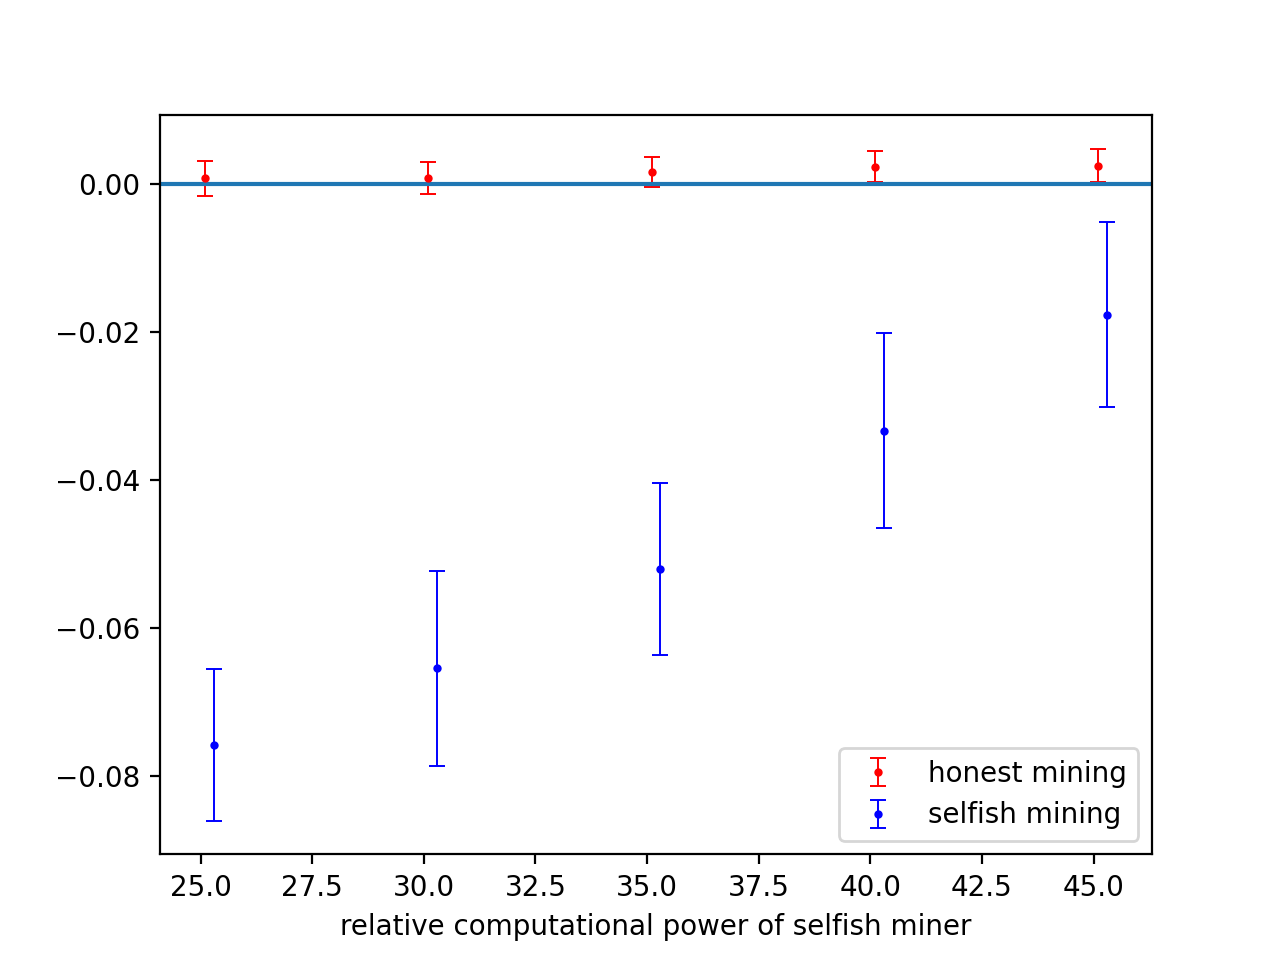
\includegraphics[width=\textwidth]{figures/multi_hr_sm_gain.png}
	\caption{Revenue and blockproduction with standard deviation for peer $0$ executing selfish mining for various relative hashrates}
	\label{fig:multi_hr}
\end{figure}
Figure~\ref{fig:multi_hr} shows the revenue gain for $25\% $, $30\%$, $35\% $, $40\% $ and $45\% $ relative compuational power. Figure~\ref{fig:multi_hr} shows that for selfish mining the revenue gain is strictly below zero, while for honest mining it is above zero. This shows that in this scenario honest mining is outperforming selfish mining. Increasing the relative computational power also increases revenue gain for the selfish miner. In contrast the small revenue gain of the honest miner remains constant. Looking at the standard deviation the revenue gain seems to be wide spread. Nonetheless, this contradicts the results of \cauth{eyal} since they showed a strict revenue increase for $\alpha > 33\% $. Since $\alpha$ can be seen as the fraction of blocks a miner produces it is directly linked to the relative computational power this miner possesses. Thus, according to \cauth{eyal} Figure~\ref{fig:multi_hr} should be positive for the relative compuational power greater than $33\% $.



\newpage
\textcolor{red}{Ab hier, TODO}
\subsection{Selfish Mining with Networking Advantage}

topological advantage, and "bandwidth"

"trying to make selfish mining work"
\subsection{On Achievability of Networking Advantage}
betweeness centrality discussion
\subsection{Selfish Mining and Global Network Characteristics}
vllt das ans ende?	

mainly focus on growth? growth analyse war leider bisher etwas enttäuschend

This section will analyze how global system behavior changes when peers executing selfish mining are introduced to the system. In Section~\ref{gopalananalysis} the Simpy Blockchain Simulator was verified against the results published by \gopalan. \gopalan analyzed the blockchain system from a global perspective using metrices based on growth and block propagation. Thus, those base metrices will be first used to analyze the global state with adversarial miners.

\textcolor{red}{TODO: vgl. zwischen sm und nicht etc.}

Selfish mining leads to intentional forks in the blockchain.

  






\subsection{Networking effects impacting selfish mining}
Central to this thesis remains the question how impactful network effects are on the performance of selfish mining. The comparison of local and global factors from a single peer point of view can be utilized to describe a networking advantage this peer possesses.
Selfish mining is executed in order to gain revenue. Revenue gain can be measured by comparing the actual revenue to the relative computational power of the peer.
\subsubsection{Computational Power and Selfish Mining}


\subsubsection{Network Advantage and Selfish Mining}
Key aspects determining networking characteristics of a specific peer are his location relative to the network and his bandwidth, while key factors on a global scale are topology, network size and bandwidth distribution, as described in Table~\ref{keyfactors}. If for example all peers in the network possess the same amount of bandwidth, increasing the bandwidth of the selfish miner will put him at a network advantage.
If the network topology is described as a $k$-random regular graph, then allowing the selfish miner to connect to more then $k$ peers will result in a networking advantage. This topological factor can be measured by graph metrices, such as betweeness centrality.

\paragraph{Betweeness Centrality}
If revenue gain is positively correlated to network advantage, than a goal of a selfish miner should be to increase his network advantage. As discussed before one can analyze the resulting networking advantage utilizing network metrices such as betweeness centrality.
\begin{figure}[ht]
	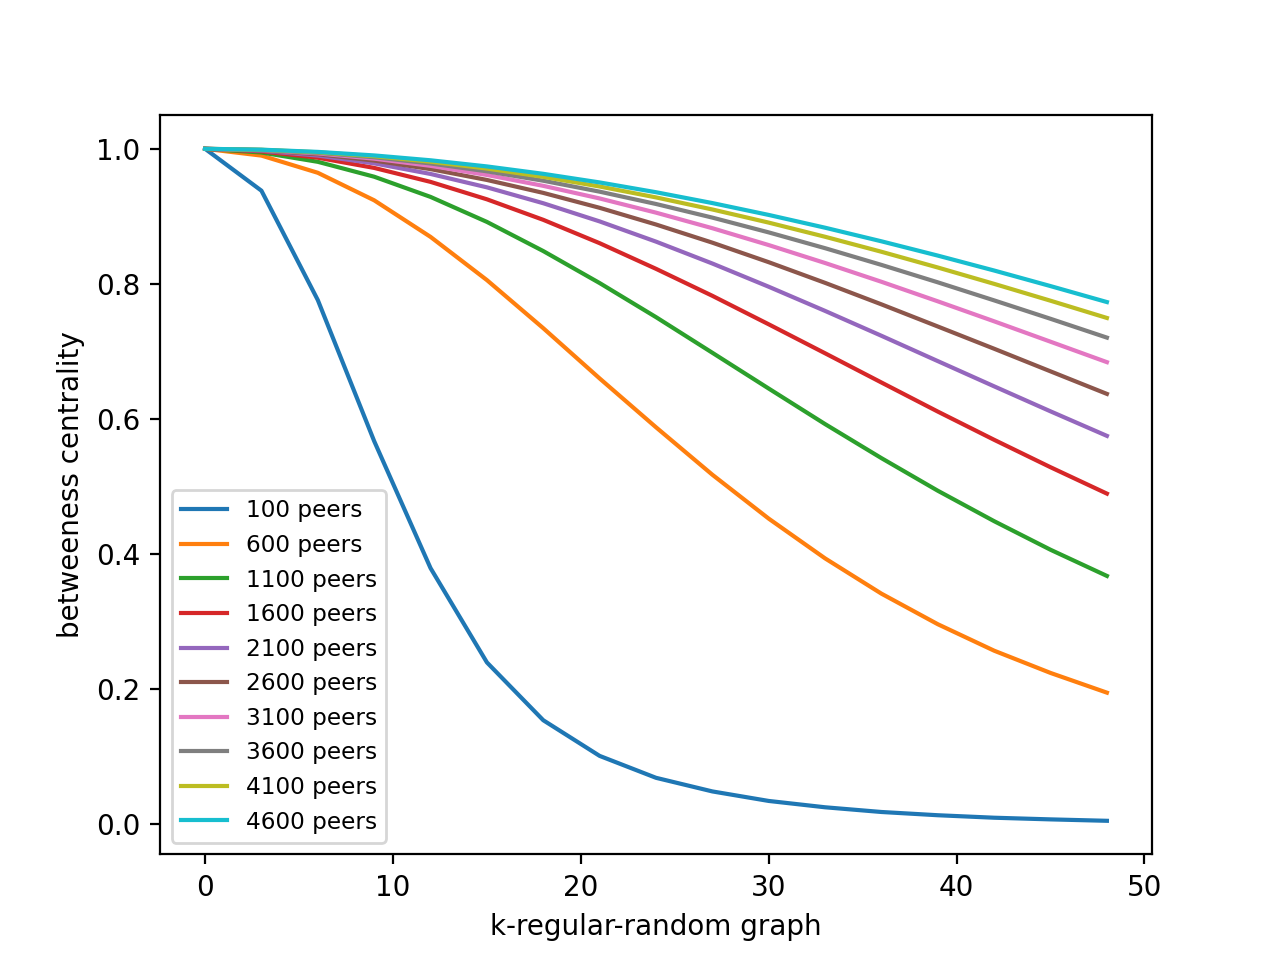
\includegraphics[width=\textwidth]{figures/betweeness_centrality.png}
	\caption{Betweeness centrality for various k-random-regular graphs for an all-connected peer $0$}
	\label{fig:bet_cent}
\end{figure}
Figure~\ref{fig:bet_cent} visualizes the betweeness centrality of one peer in various k-random-regular graphs. This specific peer, peer $0$, is connected to all other nodes. The rest of the graph follows a random-regular structure. The x-axis visualizes the increasing $k$ of the k-random-regular graph. As $k$ increases the betweeness centrality of peer $0$ decreases. For smaller node amounts the decrease is faster than for bigger node amounts. This is due to the absolut increase in $k$ since a 20-regular-random graph of 100 peers is better connected than a 20-regular-random graph of 1100 peers. Better connected means in this case it is closer to a fully connected graph. The closer the graph gets to being fully connected the more the central role of peer $0$ decreases, since the number of alternative paths between any other two peers rises. Nonetheless, Figure~\ref{fig:bet_cent} shows the upper limit for peer $0$. This means that in general a peer has to connect to a large amount of peers, compared to the network average in order to obtain any networking advantage.

\subsubsection{Topological Networking Advantage}
It can be assumed that a peer with a higher degree than the network average possesses a networking advantage. Thus, raising the degree of the selfish miner puts him at a topological networking advantage. We can then estimate the actual networking advantage based on the betweeness centrality and $\gamma$ of the peer. 
\begin{figure}[ht]
		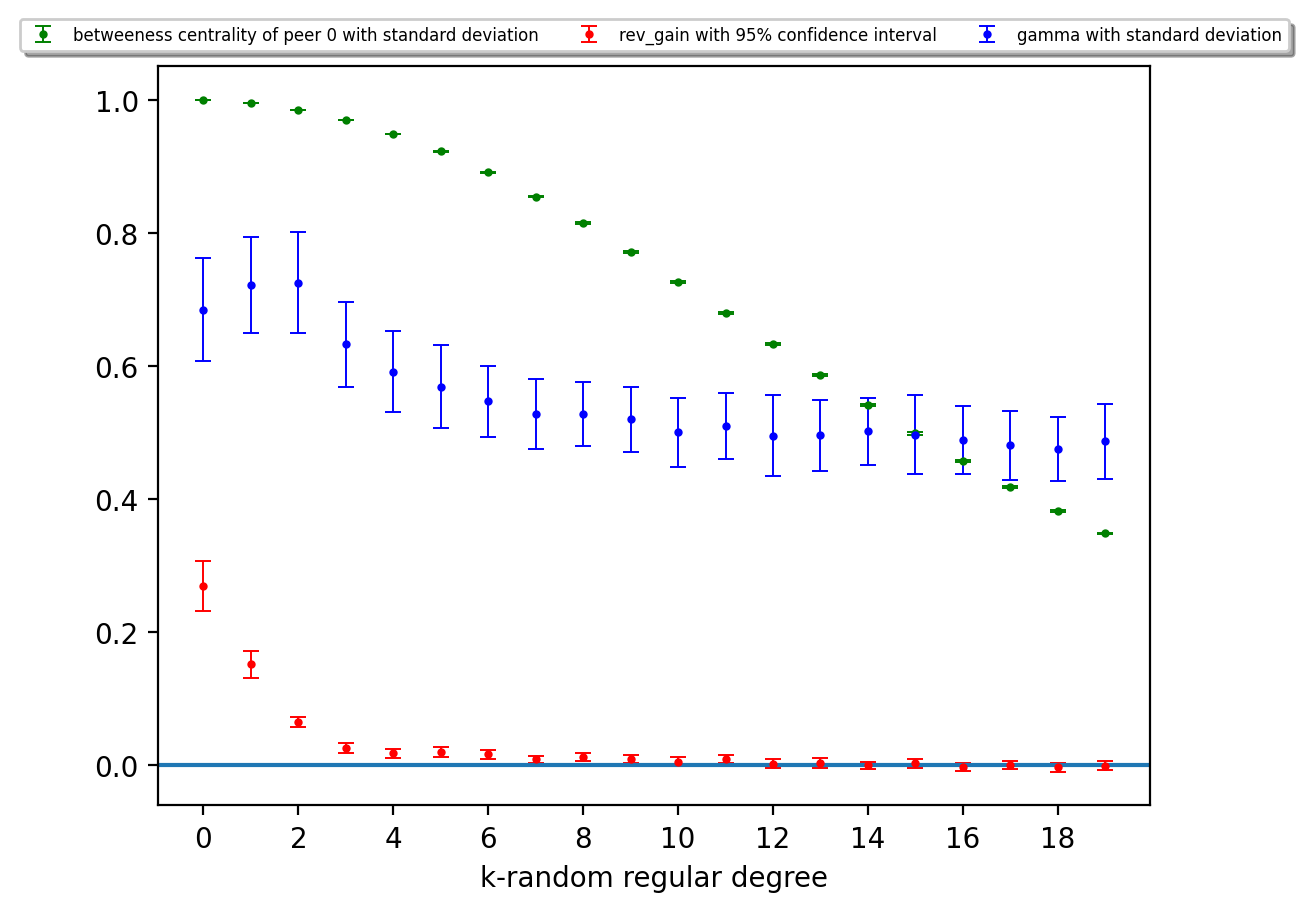
\includegraphics[width=\textwidth]{figures/full_sm_multi_degree_200rev_and_bpr_per_peer.png}
		
\caption{Betweeness Centrality, Revenue Gain and Network Propagation Factor, Topological Advantage Simulations with 200 Peers}
\label{fig:top_adv200}
\end{figure}

Figure~\ref{fig:top_adv200} shows results of experiments, which were based on analyzing the impact of topological network advantage. The experiments were carried out with 100, 200 and 300 peers respectively. Figure~\ref{fig:top_adv200} shows the results of the simulations for 200 peers, since no significant difference could be observed between 100, 200 and 300 peers simulations. The selfish miner possessed a relative computational power of $45\% $ while the rest was exponentially distributed on the remaining network. The interarrival time for communication process events was set to $1s$. The interarrival time for the block arrival process was set to $100s$. The selfish miner was connected to all peers. The rest of the network topology formed a $k$-random-regular graph, with an increasing $k$ shown in the x-axis.

The green bars represent the betweeness centrality of the selfish miner. The betweeness centrality of the selfish miner decreases as $k$ increases. The blue bar represents $\gamma$. We can observe that for each categroy of peer amounts $\gamma$ is slightly highest for $k \in \{0,1,2\}$ and is rather constant for $k>2$. $\gamma$  constant at around $0.55$ even though the betweeness centrality drops for increasing $k$'s. Thus, it is likely that $\gamma$ and  betweeness centrality are not correlated.

We can further observe that the revenue gain, shown in red, is highest for $k=0$. This is understandable since at $k=0$ the selfish miner can effectively eclipse every peer. The selfish miner is in total control over the information flow. For $k=1$ and $k=2$ revenue gain begins decreasing towards $0$ revenue gain. At $k=1$ and $k=2$ the selfish miner can still eclipse parts of the network but since overall connectedness increases, it becomes harder for the selfish miner to effectively eclipse every peer in the network. For $k>2$ revenue gain still seems to be slightly above $0$ which suggests that selfish mining is profitable.























\chapter{Conclusion}\label{chap:conclusion}


\backmatter

\cleardoublepage

\backmatter
\bibliography{references.bib}
    
\end{document}
